% !TeX program = /Library/TeX/texbin/xelatex
% !BIB program = /Library/TeX/texbin/biber
% 东北大学本科生毕业设计（论文）LaTeX稿（按学校模板与示例论文结构整理）
% 说明：
% 1. 本稿已按“封面—中英文摘要—目录—正文—参考文献—附录—致谢”组织。
% 2. 已结合你的项目：中文虚假评论检测、细粒度 claim 分析、元数据辅助、多域泛化。
% 3. 文中用 [TODO] 明确标出你需要补充的实验结果、图、表、指导教师等信息。

\documentclass[UTF8,oneside,openright,fontset=none]{ctexbook}

% =========================
% 基础宏包
% =========================
\usepackage[a4paper,top=2.5cm,bottom=2.5cm,left=3.0cm,right=2.5cm,headheight=15pt,headsep=0.8cm,footskip=1.2cm]{geometry}
\usepackage{fontspec}
\usepackage{xeCJK}
\usepackage{graphicx}
\usepackage{array}
\usepackage{booktabs}
\usepackage{longtable}
\usepackage{tabularx}
\usepackage{multirow}
\usepackage{caption}
\usepackage{subcaption}
\usepackage{amsmath,amssymb,bm}
\usepackage{tikz}
\usetikzlibrary{positioning}
\usepackage{fancyhdr}
\usepackage{titlesec}
\usepackage{titletoc}
\usepackage{tocloft}
\usepackage{indentfirst}
\usepackage{enumitem}
\usepackage{xcolor}
\usepackage{url}
\usepackage[hidelinks]{hyperref}
\usepackage[backend=biber,style=gb7714-2015,gbnamefmt=lowercase]{biblatex}
\addbibresource{refs.bib}
\renewcommand*{\bibfont}{\songti\zihao{-4}}
\defbibheading{bibliography}[\bibname]{%
  \cleardoublepage
  \phantomsection
  \addcontentsline{toc}{chapter}{#1}
  \markboth{#1}{#1}
  \begin{center}
    \vspace*{0.8\baselineskip}
    {\heiti\zihao{-2} #1\par}
    \vspace{0.5\baselineskip}
  \end{center}
}

% =========================
% 字体与字号（按学校模板近似实现）
% =========================
\setmainfont{Times New Roman}
\setsansfont{Arial}
\setmonofont{Courier New}
% \setCJKmainfont{Songti SC}
\setCJKmainfont[BoldFont=Songti SC Bold]{Songti SC}
\setCJKfamilyfont{zhsong}[BoldFont=Songti SC Bold]{Songti SC}
\setCJKfamilyfont{zhhei}{Heiti SC}

\setCJKsansfont{Heiti SC}
\setCJKmonofont{Songti SC}
\providecommand{\songti}{\CJKfamily{zhsong}}
\providecommand{\heiti}{\CJKfamily{zhhei}}

% 学校模板要求正文为宋体小四、固定值23磅；LaTeX中近似实现
\linespread{1.32}
\setlength{\parindent}{2em}
\setlength{\parskip}{0pt}

% =========================
% 图表、公式编号
% =========================
\numberwithin{equation}{chapter}
\renewcommand{\theequation}{\thechapter.\arabic{equation}}
\renewcommand{\thefigure}{\thechapter.\arabic{figure}}
\renewcommand{\thetable}{\thechapter.\arabic{table}}
\captionsetup[figure]{font=small,labelsep=space}
\captionsetup[table]{font=small,labelsep=space}

% =========================
% 页眉页脚
% =========================
\pagestyle{fancy}
\fancyhf{}
\fancyhead[L]{\songti\zihao{5} 东北大学课程报告}
\fancyhead[R]{\songti\zihao{5} \nouppercase{\leftmark}}
\fancyfoot[C]{\rmfamily\zihao{5} \thepage}
\renewcommand{\headrulewidth}{0.4pt}
\renewcommand{\footrulewidth}{0pt}

\fancypagestyle{frontmatterstyle}{
  \fancyhf{}
  \fancyhead[L]{\songti\zihao{5} 东北大学课程报告}
  \fancyhead[R]{\songti\zihao{5} \nouppercase{\leftmark}}
  \fancyfoot[C]{\rmfamily\zihao{5} \thepage}
  \renewcommand{\headrulewidth}{0.4pt}
}

\fancypagestyle{mainmatterstyle}{
  \fancyhf{}
  \fancyhead[L]{\songti\zihao{5} 东北大学课程报告}
  \fancyhead[R]{\songti\zihao{5} \nouppercase{\leftmark}}
  \fancyfoot[C]{\rmfamily\zihao{5} \arabic{page}}
  \renewcommand{\headrulewidth}{0.4pt}
  \renewcommand{\footrulewidth}{0pt}
}

\fancypagestyle{plain}{
  \fancyhf{}
  \fancyhead[L]{\songti\zihao{5} 东北大学课程报告}
  \fancyhead[R]{\songti\zihao{5} \nouppercase{\leftmark}}
  \fancyfoot[C]{\rmfamily\zihao{5} \thepage}
  \renewcommand{\headrulewidth}{0.4pt}
  \renewcommand{\footrulewidth}{0pt}
}

\renewcommand{\chaptermark}[1]{\markboth{#1}{}}

% =========================
% 章节标题格式
% =========================
\titleformat{\chapter}[hang]
  {\centering\heiti\zihao{-2}}
  {\thechapter}
  {1em}
  {}
\titlespacing*{\chapter}{0pt}{0pt}{18pt}

\titleformat{\section}[hang]
  {\heiti\zihao{4}}
  {\thesection}
  {0.8em}
  {}
\titlespacing*{\section}{0pt}{12pt}{8pt}

\titleformat{\subsection}[hang]
  {\heiti\zihao{-4}}
  {\thesubsection}
  {0.8em}
  {}
\titlespacing*{\subsection}{0pt}{10pt}{6pt}

\titleformat{\subsubsection}[hang]
  {\heiti\zihao{-4}}
  {\thesubsubsection}
  {0.8em}
  {}
\titlespacing*{\subsubsection}{0pt}{8pt}{4pt}

% =========================
% 目录格式
% =========================
\renewcommand{\contentsname}{目\quad 录}
\renewcommand{\cftchappagefont}{\normalfont}
\renewcommand{\cftchapfont}{\heiti\zihao{4}}
\renewcommand{\cftsecfont}{\songti\zihao{-4}}
\renewcommand{\cftsubsecfont}{\songti\zihao{-4}}
\setlength{\cftbeforechapskip}{4pt}

% =========================
% 列表环境
% =========================
\setlist[itemize]{leftmargin=2em}
\setlist[enumerate]{leftmargin=2.5em}

% =========================
% 自定义命令
% =========================
\newcommand{\TODO}[1]{\textcolor{red}{[TODO: #1]}}
\newcommand{\studentid}{20235870}
\newcommand{\classinfo}{计算机2305}
\newcommand{\schoolname}{东北大学}
\newcommand{\college}{计算机科学与工程学院}
\newcommand{\major}{计算机科学与技术}
\newcommand{\thesistitle}{基于细粒度评价单元与元数据感知的虚假餐厅评论检测研究}
\newcommand{\englishtitle}{Chinese Fake Review Detection Based on Fine-grained Claim Modeling and Metadata Fusion}
\newcommand{\authorname}{王稳淞}
\newcommand{\supervisor}{卢炳先}
\newcommand{\submitdate}{2026年6月}

\newcommand{\zhkeywords}{虚假评论检测；中文评论；细粒度声明；元数据融合；Random Forest；RoBERTa}
\newcommand{\enkeywords}{fake review detection; Chinese reviews; fine-grained claims; metadata fusion; restaurant reviews}

% =========================
% 封面
% =========================
\newcommand{\makecover}{
\begin{titlepage}
  \thispagestyle{empty}
  \vspace*{0.6cm}

  \noindent
  {\heiti\zihao{5} 学号\underline{\makebox[4.2cm][c]{20235870}} \hfill 班级\underline{\makebox[4.2cm][c]{计算机2305}}}
  % \noindent
  % {\heiti\zihao{5} 学号\underline{\makebox[4.2cm][l]{2025xxxxxx}} \hfill 密级\underline{\makebox[4.2cm][l]{公开}}}


  \vspace{2.8cm}

  \begin{center}
    {\songti\bfseries\zihao{1} 东北大学课程报告\par}
    \vspace{2.8cm}
    {\heiti\zihao{2} \thesistitle\par}
  \end{center}

  \vfill

  \begin{center}
    \renewcommand{\arraystretch}{1.8}
    \begin{tabular}{p{4cm}p{7.5cm}}
      {\songti\zihao{-3} 学\hspace{1em}院\hspace{1em}名\hspace{1em}称：} & {\songti\zihao{-3} \college} \\
      {\songti\zihao{-3} 专\hspace{1em}业\hspace{1em}名\hspace{1em}称：} & {\songti\zihao{-3} \major} \\
      {\songti\zihao{-3} 学\hspace{1em}生\hspace{1em}姓\hspace{1em}名：} & {\songti\zihao{-3} \authorname} \\
      {\songti\zihao{-3} 指\hspace{1em}导\hspace{1em}教\hspace{1em}师：} & {\songti\zihao{-3} \supervisor} \\
    \end{tabular}
  \end{center}

  \vspace{2cm}
  \begin{center}
    {\songti\zihao{3} \submitdate\par}
  \end{center}
\end{titlepage}
}

% =========================
% 学术声明
% =========================
\newcommand{\makestatement}{
\cleardoublepage
\thispagestyle{empty}
\begin{center}
  {\songti\bfseries\zihao{2} 郑\quad 重\quad 声\quad 明}
\end{center}

\vspace{1.5cm}

{\songti\zihao{4}
本人呈交的学位论文，是在导师的指导下，独立进行研究工作所取得的成果，所有数据、图片资料真实可靠。尽我所知，除文中已经注明引用的内容外，本学位论文的研究成果不包含他人享有著作权的内容。对本论文所涉及的研究工作做出贡献的其他个人和集体，均已在文中以明确的方式标明。本学位论文的知识产权归属于培养单位。}

\vspace{2.5cm}

\begin{flushright}
{\songti\zihao{4}
本人签名：\underline{\hspace{4cm}}\\[1.2cm]
日期：\underline{\hspace{4cm}}}
\end{flushright}
}

% =========================
% 中英文摘要
% =========================
\newcommand{\makezhabstract}{
\cleardoublepage
\pagestyle{frontmatterstyle}
\chapter*{摘\quad 要}
\markboth{摘要}{摘要}
\addcontentsline{toc}{chapter}{摘要}

在线评论已成为消费者进行餐饮消费决策的重要信息来源，但虚假评论的大量存在会误导用户判断、扰乱平台秩序并削弱评论系统的可信度。针对中文虚假餐厅评论检测中存在的整句级文本表示难以刻画局部证据、评论元数据利用不足等问题，本文以大众点评餐厅评论数据为研究对象，提出一种融合细粒度评价单元建模与元数据辅助判断的虚假评论检测方法。

该方法首先利用预训练RoBERTa模型提取评论的全局语义表示，并将评论划分为多个语义片段，通过可学习查询向量从分句级表示中抽取细粒度评价单元，以刻画评论中的局部证据、表达模式及潜在异常信息。在此基础上，进一步引入评分信息、交互统计、发布时间、图片数量及文本统计特征等元数据，构建元数据辅助分支，并结合随机森林生成的元数据专家分数，实现全局文本语义、细粒度评价单元表示与元数据特征的联合融合，从而增强模型对复杂虚假评论模式的识别能力。

实验结果表明，所提出方法在大众点评虚假餐厅评论检测任务上取得了较好的分类性能。在十折交叉验证设置下，模型的平均Accuracy、Precision、Recall和F1分别达到92.72\%、93.40\%、91.99\%和92.66\%，AUC达到97.91\%，AP达到97.96\%。与传统机器学习方法和纯文本预训练模型相比，细粒度评价单元建模能够更有效地识别评论中模板化表述、夸张堆砌以及情绪结论与细节证据不一致等局部异常现象；元数据辅助分支和元数据专家分数则进一步提高了模型对可疑评论行为模式的判别能力，从而提升了整体检测效果和结果稳定性。

本文研究表明，细粒度评价单元建模与元数据融合能够有效提升中文虚假餐厅评论检测的性能与可解释性，为后续开展商家级风险评估、多模态评论分析及生成式虚假评论检测研究提供了参考。

\vspace{1em}
\noindent{\heiti\zihao{-4} 关键词：}{\songti\zihao{-4} 虚假评论检测；大众点评；细粒度评价单元；元数据融合；餐厅评论}
}

\newcommand{\makeenabstract}{
\cleardoublepage
\pagestyle{frontmatterstyle}
\chapter*{ABSTRACT}
\markboth{ABSTRACT}{ABSTRACT}
\addcontentsline{toc}{chapter}{ABSTRACT}

Online reviews have become an important source of information for consumers when making dining decisions. However, the widespread presence of fake reviews misleads users, disrupts platform order, and undermines the credibility of review systems. To address the limitations of coarse-grained sentence-level text representation and insufficient utilization of review metadata in Chinese fake restaurant review detection, this thesis focuses on Dianping restaurant review data and proposes a fake review detection method that integrates fine-grained review unit modeling with metadata-assisted classification.

The proposed method first employs a pretrained RoBERTa model to extract global semantic representations of review texts. Each review is then divided into multiple semantic segments, and several fine-grained review units are extracted from clause-level representations through learnable query vectors to characterize local evidence, expression patterns, and potentially suspicious information within the review. On this basis, metadata features including rating information, interaction statistics, posting time, picture count, and text-related statistical features are further introduced through a metadata-assisted branch. In addition, a metadata expert score generated by a random forest model is incorporated to jointly fuse global textual semantics, fine-grained review unit representations, and metadata features, thereby improving the model's ability to identify complex deceptive patterns.

Experimental results show that the proposed method achieves strong performance on Dianping fake restaurant review detection. Under a 10-fold cross-validation setting, the model obtains an average Accuracy of 92.72\%, Precision of 93.40\%, Recall of 91.99\%, and F1-score of 92.66\%, with an AUC of 97.91\% and an AP of 97.96\%. Compared with traditional machine learning methods and text-only pretrained baselines, fine-grained review unit modeling more effectively captures local anomalies such as templated expressions, exaggerated descriptions, and inconsistencies between emotional conclusions and supporting details. Meanwhile, the metadata-assisted branch and metadata expert score further improve the identification of suspicious behavioral patterns, leading to better overall detection performance and stability.

The study demonstrates that integrating fine-grained review unit modeling with metadata fusion can effectively improve both performance and interpretability in Chinese fake restaurant review detection, and provides a useful basis for future research on merchant-level risk assessment, multimodal review analysis, and AI-generated fake review detection.

\vspace{1em}
\noindent{\bfseries Keywords: }fake review detection; Dianping; fine-grained review units; metadata fusion; restaurant reviews
}

% =========================
% 目录
% =========================
\newcommand{\makemytableofcontents}{
\cleardoublepage
\pagestyle{frontmatterstyle}
\markboth{目录}{目录}
\tableofcontents
}

\begin{document}

\pagenumbering{gobble}
\makecover

\frontmatter
\makezhabstract
\makeenabstract
\makemytableofcontents

\mainmatter
\pagenumbering{arabic}
\setcounter{page}{1}
\pagestyle{mainmatterstyle}

% ==================================================
% 第1章 绪论
% ==================================================
\chapter{绪论}

\section{课题研究背景及意义}
随着电子商务平台和本地生活服务平台的快速发展，用户评论已成为影响消费决策的重要依据。无论是商品购买还是线下餐饮选择，大量用户都会在下单前参考历史评论，以评估产品质量、服务水平与性价比。然而，评论系统在带来信息透明化的同时，也为虚假评论的生成与传播提供了空间。所谓虚假评论，通常是指并非基于真实消费体验、而是出于利益驱动、人为操纵或误导性目的而发布的评论内容。其存在不仅影响普通用户对商家和商品的判断，也会破坏平台的公平竞争环境。

当前，虚假评论在中文互联网场景中具有较强的现实性。一方面，本地生活平台与电商平台上的评论数量极大，人工审查成本高；另一方面，虚假评论的写作方式正从早期的粗糙模板化向更自然、更隐蔽的表达演化，使得仅靠人工规则和浅层统计特征难以取得理想效果。尤其是在生成式人工智能不断普及的背景下，机器生成评论能够模仿真实用户语言风格，进一步提高了虚假评论检测的难度。

\begin{figure}[htbp]
  \centering
  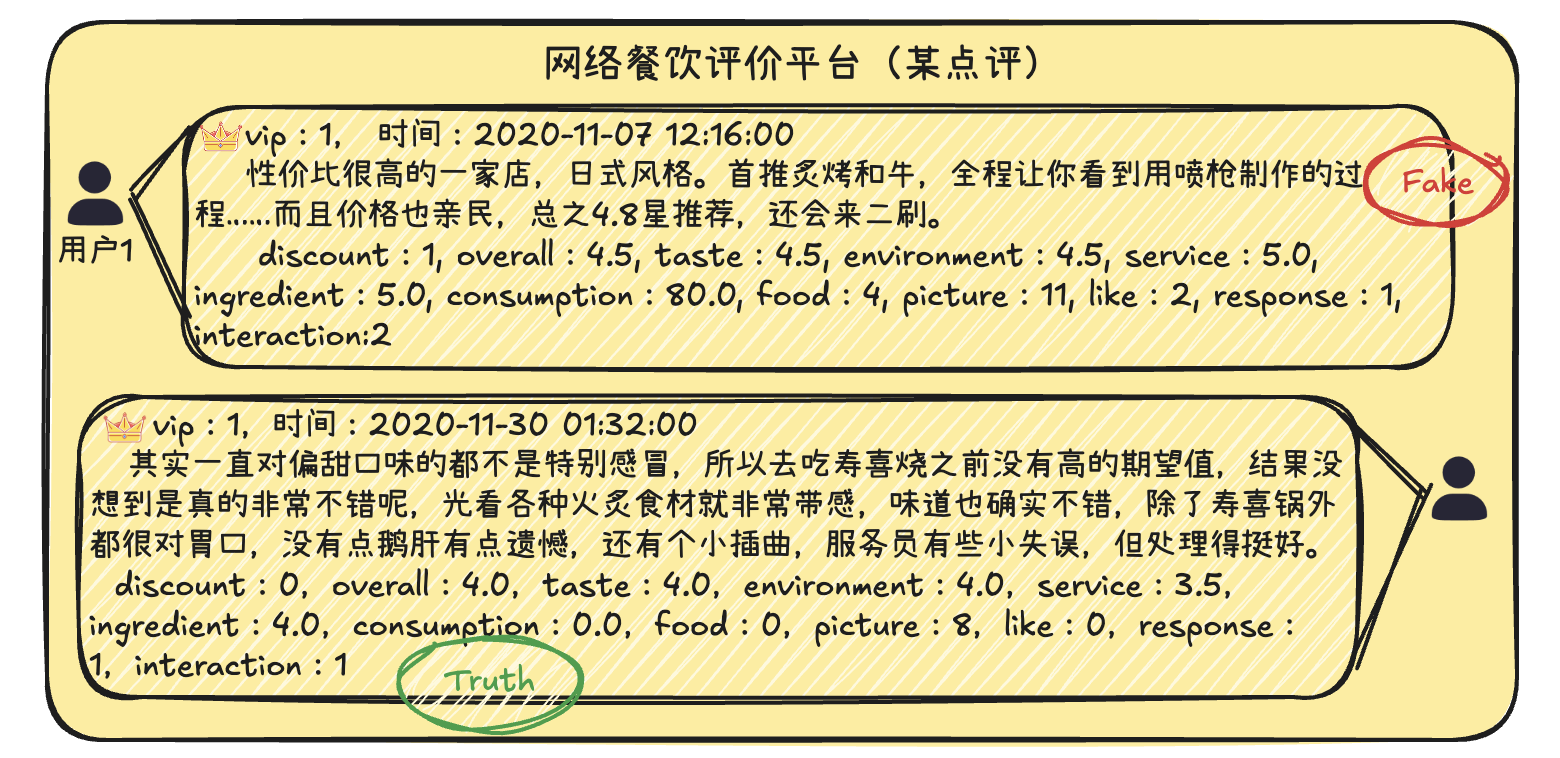
\includegraphics[width=0.8\textwidth]{figures/dianping.png}
  \caption{网络餐饮评论示例}
  \label{fig:dianping}
\end{figure}

从研究角度看，虚假评论检测既是自然语言处理中的文本分类问题，也是一个与平台治理、商业生态和消费者权益保护密切相关的应用问题。对于中文场景而言，该任务还面临数据资源不足、领域差异显著、元数据利用不充分等难点。因此，研究更适合中文评论语料特点、同时兼顾性能、可解释性与泛化能力的虚假评论检测方法，具有较强的理论价值和实际意义。

本文以中文虚假餐厅评论检测为研究对象，围绕“如何从评论内部的细粒度表达结构中挖掘更有判别力的语义信息，并利用可获得元数据增强模型判断能力”这一问题展开研究。希望通过引入细粒度评价单元建模与元数据融合机制，提高模型对虚假评论的识别效果，并为后续开展商家级风险分析、多模态扩展与生成式虚假评论检测研究提供方法基础。



\section{国内外研究现状}
\subsection{传统机器学习方法}
虚假评论检测早期研究主要依赖人工特征工程与传统分类器，例如朴素贝叶斯、逻辑回归、支持向量机与决策树等。这类方法通常围绕文本长度、情感词比例、词频分布、用户行为特征与时间统计特征进行建模，具有实现简单、训练高效的优点。但由于其性能高度依赖人工设计特征，难以充分学习评论文本中的深层语义结构，面对表达更自然、更复杂的虚假评论时容易出现性能瓶颈。

\subsection{图结构与关系建模方法}
为利用评论、用户、商家及交互关系之间的结构信息，部分研究将虚假评论检测建模为图分析或异构信息网络问题。该类方法能够从实体之间的关联中挖掘异常模式，例如刷评团体、异常交互链路与可疑用户群体等，在某些数据集上具有较好表现。然而，其有效性往往依赖较完整的关系数据与较强的图结构先验，在真实中文评论平台场景中，这类信息并不总是充分可用。

\subsection{深度学习与预训练模型方法}
随着深度学习和预训练语言模型的发展，越来越多研究采用 CNN、RNN、BERT 及其变体来处理虚假评论检测任务。与传统方法相比，这类模型能够自动学习上下文相关表示，更适合处理文本语义复杂、模式隐蔽的评论内容。已有研究表明，基于 Transformer 的模型在评论分类任务中表现出较强能力，但不少方法仍以整条评论的粗粒度表示为主，对评论内部的局部语义片段、论证结构和可疑表达模式挖掘不足。

\subsection{元数据融合研究}
在餐饮评论虚假检测场景中，评论文本并不是唯一的信息来源。评分、时间、交互量、用户属性、商家回复等元数据往往也包含重要的判别信号。参考文献中提供的餐饮虚假评论研究表明，构建丰富元数据特征并与文本表示进行融合，能够显著提升模型表现；其提出的数据集包含丰富元数据，并将 Transformer 文本表示、TextCNN 情感表示与带注意力的 MLP 特征融合在一起，取得了较好的准确率和泛化结果。这说明在评论检测任务中，文本与元数据联合建模具有明确价值。


\subsection{现有工作的不足}
综合来看，现有研究仍存在以下不足：
\begin{enumerate}
  \item 中文虚假评论研究相较英文场景仍不充分，公开可复用的数据与成熟基线相对较少；
  \item 大量方法使用整体文本表示进行二分类，忽略了评论内部细粒度语义片段之间的差异；
  \item 元数据在不少中文实验中没有被系统利用，导致模型鲁棒性与泛化能力受限；
  \item 针对模型判别依据的解释能力关注不足，不利于进一步开展风险分析和实际应用。
\end{enumerate}

因此，围绕中文评论场景，构建一种“细粒度文本建模 + 元数据辅助判断”的检测框架，具有较强研究价值。

\section{可行性分析}
本文工作的可行性主要体现在以下几个方面。

首先，在数据基础方面，本文已经具备开展中文虚假餐厅评论检测实验所需的数据条件，并已完成大众点评评论数据的读取、清洗、字段整理与特征构建，可支持模型训练、对比实验与消融分析。

其次，在方法基础方面，本文已经完成基于中文预训练模型的评论分类实验，并初步实现了细粒度评价单元抽取与元数据融合相关模块，具备继续开展模型完善、实验验证与论文写作的实现条件。

再次，在实验基础方面，本文已能够使用 HuggingFace Transformers、PyTorch 等工具完成模型训练、评估与结果分析；同时，已获得随机森林、纯文本 RoBERTa 等基线结果，可为后续论文中的对比实验提供支撑。

最后，在研究创新性方面，本文并非停留于简单二分类，而是尝试从评论内部语义结构入手进行细粒度建模，并结合元数据增强判断能力。这一思路既与已有元数据融合研究形成呼应，又能够体现自身的模型设计特色与中文餐饮评论场景的适配价值。

\section{本文主要工作}
本文围绕中文虚假餐厅评论检测任务，开展了以下几个方面的研究工作：

\subsection{本文的研究内容}
\begin{enumerate}
  \item 对大众点评中文餐厅评论数据进行整理和统一表示，构建适合实验的训练与测试数据形式；
  \item 设计基于预训练语言模型的评论编码框架，在全局文本表示基础上进一步引入细粒度评价单元抽取机制，以建模评论内部的局部语义片段；
  \item 构建元数据辅助分支，将可获得的结构化特征与文本表征进行融合，并引入随机森林元数据专家分数，增强模型对可疑评论模式的识别能力；
  \item 设计并完成多组实验，包括基线对比实验、消融实验、阈值搜索实验以及可解释性分析，用于验证各个模块的有效性；
  \item 对模型结构、训练过程、实验结果和不足进行系统分析，为后续研究提供参考。
\end{enumerate}

\subsection{技术路线}
本文的技术路线如下：首先，对大众点评评论数据进行清洗、标签整理、字段统一和特征构建，形成适合模型训练的统一输入形式；其次，利用预训练语言模型对评论文本进行编码，并在此基础上进行分句处理，通过可学习查询向量从分句级表示中抽取多个细粒度评价单元，以获得评论内部的局部证据表示；然后，将评分、时间、交互、图片及统计特征输入元数据辅助分支，同时构建随机森林元数据专家分数，为模型提供额外的结构化判别信息；最后，将全局文本表示、细粒度评价单元表示、元数据高层表示及专家分数进行联合融合，完成虚假评论分类，并通过基线对比实验、消融实验、阈值搜索实验和可解释性分析对模型性能进行评估。

\section{本文组织结构}
本文共分为五章，各章内容安排如下：

第1章为绪论，介绍课题背景、国内外研究现状、研究意义、可行性分析以及本文主要工作。

第2章介绍相关理论与关键技术，包括中文预训练语言模型、细粒度评价单元建模思想、元数据特征构建方式以及相关评价指标。

第3章给出本文所提出的中文虚假评论检测模型设计，包括整体框架、文本编码模块、细粒度评价单元抽取模块、元数据辅助分支及最终融合分类器。

第4章介绍实验设计与结果分析，包括数据集说明、实验环境、对比实验、消融实验、阈值搜索实验和可解释性展示。

第5章总结全文工作，并对后续可进一步研究的方向进行展望。

% ==================================================
% 第2章 相关理论与技术
% ==================================================
\chapter{相关理论与技术}

\section{任务定义}
本文研究的中文虚假评论检测任务本质上属于监督式文本分类问题。设评论文本为 $x$，其对应的元数据特征向量为 $m$，标签为 $y\in\{0,1\}$，其中 $0$ 表示真实评论，$1$ 表示虚假评论，则目标是学习一个分类函数
\begin{equation}
  \hat{y} = f(x,m;\theta),
\end{equation}
其中 $\theta$ 表示模型参数，$\hat{y}$ 表示模型预测结果。

与仅使用整条评论全局表示的传统文本分类不同，本文进一步将评论分解为多个语义片段，并通过细粒度声明建模获得局部证据表示。设一条评论被划分为 $n$ 个片段，记为
\begin{equation}
  x = \{c_1,c_2,\ldots,c_n\},
\end{equation}
则模型不仅需要学习整体评论的语义，还需要关注各片段在虚假评论识别中的不同贡献。

\section{中文预训练语言模型}
预训练语言模型通过在大规模语料上进行自监督学习，能够获得具有上下文语义信息的文本表示。在中文评论检测任务中，预训练模型相比传统词袋模型和静态词向量方法，能够更好地捕获语义组合关系、情感倾向与上下文依赖。

本文采用中文 RoBERTa 系列模型作为文本编码主干，其基本思想是在输入评论序列后，通过多层 Transformer 编码器获得 token 级隐藏表示和句级全局表示。设输入 token 序列为
\begin{equation}
  X = [t_1,t_2,\ldots,t_L],
\end{equation}
则编码器输出为
\begin{equation}
  H = [h_1,h_2,\ldots,h_L],\quad h_i\in\mathbb{R}^{d}.
\end{equation}
通常使用特殊位置的全局向量或池化后的表示作为整条评论的全局语义特征。

\section{细粒度声明建模}
在虚假评论检测中，仅依赖评论整体表示会掩盖评论内部不同语义片段的差异。例如，一条评论可能同时包含商品描述、主观情感、物流评价和夸张修辞等多种成分，其中只有部分内容真正反映了虚假性。为提升模型对这类局部异常模式的感知能力，本文引入细粒度声明建模思想。

具体而言，先依据标点或规则将评论切分为多个候选片段，再利用可学习查询向量从 token 表示中聚合出多个声明表示。设 token 级表示矩阵为 $H\in\mathbb{R}^{L\times d}$，第 $k$ 个查询向量为 $q_k\in\mathbb{R}^{d}$，则其对应注意力权重可表示为
\begin{equation}
  \alpha_k = \mathrm{softmax}\left(\frac{Hq_k}{\sqrt{d}}\right),
\end{equation}
进一步得到第 $k$ 个声明表示
\begin{equation}
  z_k = \sum_{i=1}^{L} \alpha_{k,i} h_i.
\end{equation}
多个声明向量共同构成评论内部的细粒度语义表征，用于后续判别。

\section{元数据特征建模}
评论元数据是指除评论文本之外的辅助信息，例如评论时间、评分、点赞数、交互情况、用户信息及其他结构化属性。这类信息虽然不直接描述语义内容，但在虚假评论识别中往往具有显著价值。

对于结构化元数据，本文将其整理为固定维度特征向量
\begin{equation}
  m = [m_1,m_2,\ldots,m_p].
\end{equation}
在输入模型前，连续特征可进行标准化处理，离散特征可进行数值映射或独热编码。随后通过多层感知机得到元数据表示：
\begin{equation}
  h_m = \mathrm{MLP}(m).
\end{equation}
为增强不同特征维度的重要性建模能力，可进一步引入注意力或门控机制对元数据表示进行重加权。

\section{随机森林元数据专家分数}
除深度模型中的元数据辅助分支外，本文还引入随机森林模型生成元数据专家分数，用于补充结构化判别信息。随机森林（Random Forest）是一种典型的集成学习方法，其核心思想是通过自助采样（Bootstrap）构建多棵决策树，并对多棵树的输出结果进行集成，从而提升模型的鲁棒性与泛化能力。

相较于单一决策树，随机森林能够在保留非线性建模能力的同时，有效降低模型对局部噪声和特定特征组合的敏感性。在虚假评论检测任务中，评论评分、交互统计、时间分布、图片数量等元数据之间往往存在较复杂的非线性关系，因此随机森林能够较好地挖掘结构化特征中的判别模式。

设标准化后的元数据输入为 $m$，随机森林输出该评论属于虚假评论的概率为
\begin{equation}
  s_{\mathrm{rf}} = g(m),
\end{equation}
其中 $g(\cdot)$ 表示随机森林模型，$s_{\mathrm{rf}}$ 表示对应的元数据专家分数。该分数可视为一种基于传统机器学习视角得到的结构化先验判断，与神经网络所学习到的文本语义特征和元数据高层表示形成互补。

为避免在训练集上直接使用随机森林拟合后的概率而引入信息泄漏，本文在训练过程中采用基于交叉验证的 out-of-fold 策略生成训练集上的专家分数；对于验证集或测试集，则使用完整训练集训练得到的随机森林模型进行打分。最终，随机森林输出的一维概率分数作为额外结构化特征，与全局文本表示、细粒度声明表示及元数据表示共同输入后续融合分类器，从而增强模型对虚假评论模式的综合判别能力。

\section{NearMiss-1 欠采样策略}
虚假评论检测任务通常存在明显的类别不平衡问题，即真实评论数量远多于虚假评论数量。若直接在原始数据上训练模型，分类器容易偏向多数类，从而导致对少数类虚假评论的识别能力下降。为缓解这一问题，本文采用 NearMiss-1 欠采样策略对训练数据进行平衡处理。

NearMiss 是一种基于样本距离的欠采样方法，其基本思想是在多数类样本中选择那些与少数类样本距离较近的样本保留下来，以保留更具判别难度的边界信息。其中，NearMiss-1 的选择规则是：对于每个多数类样本，计算其到若干最近少数类样本的平均距离，并优先保留平均距离较小的多数类样本。该方法能够使保留下来的多数类样本更多分布在类别边界附近，从而提高模型对两类样本分界区域的学习能力。

设多数类样本集合为 $\mathcal{D}_{maj}$，少数类样本集合为 $\mathcal{D}_{min}$，对任一多数类样本 $x_i \in \mathcal{D}_{maj}$，NearMiss-1 根据其到最近 $k$ 个少数类样本的平均距离
\begin{equation}
  d_i = \frac{1}{k}\sum_{j=1}^{k}\mathrm{dist}(x_i, x_j^{min})
\end{equation}
进行排序，并保留平均距离较小的多数类样本，其中 $\mathrm{dist}(\cdot)$ 表示距离度量函数。通过这种方式，可在减少多数类样本数量的同时，尽可能保留靠近分类边界的有效样本信息。

结合当前实验实现，本文首先对元数据特征进行标准化处理，然后基于标准化后的特征空间执行 NearMiss-1 欠采样。若数据中存在可区分的城市字段，则优先按城市分组分别执行 NearMiss-1，以降低不同城市评论分布差异对采样结果的影响；若缺少有效城市信息，则退化为全局 NearMiss-1 欠采样。该策略能够在类别平衡与样本代表性之间取得较好的折中，为后续模型训练提供更稳定的数据基础。

\section{十折交叉验证}
为全面评估模型在虚假评论检测任务中的泛化性能，本文采用十折交叉验证（10-fold Cross Validation）作为主要实验评估方式。交叉验证是一种常用的模型评估方法，其核心思想是将数据集划分为若干互不重叠的子集，轮流使用其中一个子集作为验证集，其余子集作为训练集，从而减少由单次随机划分带来的偶然性。

具体而言，设平衡处理后的数据集为 $\mathcal{D}$，将其划分为 $10$ 个大小近似相等的子集：
\begin{equation}
  \mathcal{D}=\mathcal{D}_1\cup \mathcal{D}_2\cup \cdots \cup \mathcal{D}_{10},
\end{equation}
并满足
\begin{equation}
  \mathcal{D}_i \cap \mathcal{D}_j = \varnothing,\quad i\neq j.
\end{equation}
在第 $t$ 次实验中，取 $\mathcal{D}_t$ 作为验证集，其余 $9$ 个子集合作为训练集。重复 $10$ 次后，可得到模型在不同划分下的多组实验结果，最终取各项指标的平均值和标准差作为模型性能的综合评价。

为尽可能保持各折中类别分布的一致性，本文采用分层十折交叉验证（Stratified 10-fold Cross Validation），即在划分过程中保持真实评论与虚假评论的比例在各折中尽量一致。该策略尤其适用于类别分布不均衡的二分类任务，能够更稳定地评估模型在不同数据划分下的表现。

与单次训练/测试划分相比，十折交叉验证具有以下优点：第一，能够更充分地利用有限数据，使每个样本都至少有一次作为验证样本参与评估；第二，能够减小偶然划分带来的性能波动，使实验结果更稳定、更具说服力；第三，便于对模型的平均性能和结果方差进行分析，从而更客观地比较不同模型或不同模块的效果。因此，本文在主实验中采用十折交叉验证对模型进行系统评估。

\section{评价指标}
本文采用准确率（Accuracy）、精确率（Precision）、召回率（Recall）与 F1 值作为主要评价指标。设 TP、FP、TN、FN 分别表示真正例、假正例、真反例与假反例，则各指标定义如下：
\begin{equation}
  \mathrm{Accuracy} = \frac{TP + TN}{TP + TN + FP + FN},
\end{equation}
\begin{equation}
  \mathrm{Precision} = \frac{TP}{TP + FP},
\end{equation}
\begin{equation}
  \mathrm{Recall} = \frac{TP}{TP + FN},
\end{equation}
\begin{equation}
  \mathrm{F1} = \frac{2\times \mathrm{Precision}\times \mathrm{Recall}}{\mathrm{Precision}+\mathrm{Recall}}.
\end{equation}

其中，F1 值综合考虑了查准率与查全率，适合用于类别分布不完全均衡的虚假评论检测任务。

% % ==================================================
% % 第3章 模型设计与实现
% % ==================================================
% \chapter{模型设计与实现}

% \section{总体框架}
% 本文提出的模型总体上由四个部分组成：文本全局编码模块、细粒度声明抽取模块、元数据辅助分支和融合分类模块。整体思路如图~\ref{fig:framework} 所示。

% \begin{figure}[htbp]
%   \centering
%   \fbox{\rule{0pt}{5cm}\rule{0.82\textwidth}{0pt}}
%   \caption{本文模型总体框架示意图}
%   \label{fig:framework}
% \end{figure}

% \noindent 图~\ref{fig:framework} 建议你替换为自己绘制的结构图，图中应至少包含以下流程：
% \begin{enumerate}
%   \item 评论文本输入 RoBERTa 编码器得到 token 表示与全局表示；
%   \item token 表示进入 claim extractor 得到多个声明向量；
%   \item 元数据特征输入 MLP/注意力模块得到结构化表征；
%   \item 三类特征融合后送入分类器输出真假标签。
% \end{enumerate}

% \section{文本全局编码模块}
% 对于输入评论文本，本文首先使用中文预训练语言模型提取全局语义表示。设输入序列经过编码后得到隐藏状态矩阵 $H\in\mathbb{R}^{L\times d}$，则取首位全局向量或池化结果作为评论整体表示：
% \begin{equation}
%   h_g = \mathrm{Pool}(H).
% \end{equation}

% 全局表示能够反映评论整体语义和主观倾向，是模型进行真假判断的重要基础。但仅凭全局向量往往难以捕获评论内部局部异常模式，因此需要进一步进行细粒度建模。

% \section{细粒度声明抽取模块}
% \subsection{评论片段划分}
% 为了使模型更细致地观察评论内部结构，本文首先基于中文标点对评论进行片段划分。设一条评论被切分为若干子句或短句，这些局部片段在语义上往往承担不同功能，例如事实描述、主观感受、价格评价、物流体验等。

% 在实现中，可通过“，。！？；”等标点对文本进行规则切分，并限制最大子句数量。对于过长评论，可在截断前优先保留更具信息量的子句。

% \subsection{声明查询聚合}
% 在获得 token 表示后，本文引入多个可学习查询向量，从文本表示中抽取多个声明级表示。设共有 $K$ 个查询向量，则得到 $K$ 个声明向量：
% \begin{equation}
%   Z = [z_1,z_2,\ldots,z_K],\quad z_k\in\mathbb{R}^{d}.
% \end{equation}

% 这种方式能够使不同查询聚焦于评论中的不同语义区域，提升模型对局部可疑模式的建模能力。例如，某一声明可能集中关注夸张赞美表述，另一声明可能更关注与事实细节相关的片段。

% \subsection{声明级可疑性建模}
% 为了进一步利用声明信息，本文将各声明向量送入可疑性判别层，估计其潜在异常程度：
% \begin{equation}
%   s_k = \sigma(W_s z_k + b_s),
% \end{equation}
% 其中 $s_k$ 表示第 $k$ 个声明的可疑性得分。最后对多个声明进行聚合，得到声明级综合表示：
% \begin{equation}
%   h_c = \sum_{k=1}^{K} \beta_k z_k,
% \end{equation}
% 其中 $\beta_k$ 可由 $s_k$ 或归一化权重得到。

% \section{元数据辅助分支}
% 参考现有餐饮虚假评论研究，评论中的元数据对于提升检测效果具有重要价值。结合你当前数据情况，本文建议将可用辅助特征划分为以下几类：
% \begin{enumerate}
%   \item 时间相关特征：评论时间、下单时间、时间间隔等；
%   \item 用户相关特征：用户编号、默认用户名特征、账号行为统计等；
%   \item 交互相关特征：点赞数、回复数、额外统计量；
%   \item 平台属性特征：评分、子评分、是否图片、图片数等；
%   \item 文本统计特征：长度、标点比例、重复词比例、情感强度等。
% \end{enumerate}

% 若后续扩展到其他平台，需要明确区分不同平台可用字段；本文当前实验仅使用大众点评数据。

% 元数据输入后，通过多层感知机得到表示：
% \begin{equation}
%   h_m = \phi_2(W_2\phi_1(W_1m+b_1)+b_2),
% \end{equation}
% 其中 $\phi_1,\phi_2$ 表示非线性激活函数。

% \section{特征融合与分类器}
% 本文最终将文本全局表示 $h_g$、声明级表示 $h_c$ 与元数据表示 $h_m$ 进行拼接融合：
% \begin{equation}
%   h_f = [h_g;h_c;h_m].
% \end{equation}
% 随后通过全连接层输出二分类结果：
% \begin{equation}
%   \hat{y} = \mathrm{softmax}(W_f h_f + b_f).
% \end{equation}

% 训练时采用交叉熵损失：
% \begin{equation}
%   \mathcal{L}_{cls} = -\sum_{i=1}^{N} y_i \log \hat{y}_i.
% \end{equation}
% 若你最终保留了 diversity loss、orthogonality loss 或 gate regularization，也可写成联合损失形式：
% \begin{equation}
%   \mathcal{L} = \mathcal{L}_{cls} + \lambda_1 \mathcal{L}_{div} + \lambda_2 \mathcal{L}_{orth}.
% \end{equation}
% 这里的 $\lambda_1$ 与 $\lambda_2$ 为损失权重系数。\TODO{若最终论文不使用额外损失，请删除该式。}

% \section{模型实现细节}
% 本文模型基于 PyTorch 与 HuggingFace Transformers 实现，中文文本编码器使用 \texttt{hfl/chinese-roberta-wwm-ext}。训练时根据硬件环境选择 CUDA、MPS 或 CPU 设备，优化器采用 AdamW，分类任务损失函数采用交叉熵损失。为了提升训练稳定性，可采用分阶段训练策略：先冻结部分预训练编码器参数，仅训练声明模块与分类头；随后再进行联合微调。

% 关于实现部分，正文中应以“模块功能 + 关键设计 + 训练逻辑”为主，不宜大段粘贴源码。若确需展示核心代码，建议放在附录中，并在正文只概述关键逻辑。
% ==================================================
% 第3章 模型设计与实现
% ==================================================
\chapter{模型设计与实现}

\section{总体框架}

针对中文虚假餐厅评论检测任务中“整句级表示难以充分刻画局部异常信息、结构化元数据利用不足”的问题，本文设计了一种融合全局文本语义、细粒度评价单元表示与元数据辅助信息的多分支检测模型。整体上，模型由文本全局编码模块、细粒度评价单元抽取模块、元数据辅助分支、随机森林元数据专家分数模块以及最终融合分类模块组成。

从整体流程上看，模型首先接收评论样本文本及其对应元数据作为输入；随后，一方面利用预训练语言模型对评论全文进行编码，获得整条评论的全局语义表示；另一方面将评论按标点切分为多个分句，并在分句级表示基础上抽取若干细粒度评价单元，以建模评论内部局部证据；与此同时，结构化元数据经过注意力加权与多层感知机映射后得到高层元数据表示，随机森林模型则基于同一组元数据输出一维专家分数。最后，模型对上述多源特征进行联合融合，并输出评论真假类别。

这种设计思路与参考文献中“文本分支 + 元数据感知分支 + 融合分类”的总体框架具有一致性，即都强调文本与元数据的联合建模价值，但本文并未引入独立的 TextCNN 情感分支，而是进一步突出评论内部局部证据的建模，将细粒度评价单元抽取作为模型的重要创新组成部分。参考文献中的 TTAM 模型通过 Transformer、TextCNN 与 Attention-MLP 实现文本与 rich metadata 的融合，而本文则在中文 RoBERTa 编码基础上引入 claim 分支和随机森林专家分数，以适配当前数据与任务需求。

图~\ref{fig:framework} 给出了本文模型的总体流程示意。

\begin{figure}[htbp]
  \centering
  \IfFileExists{figures/framework_overall.png}{
    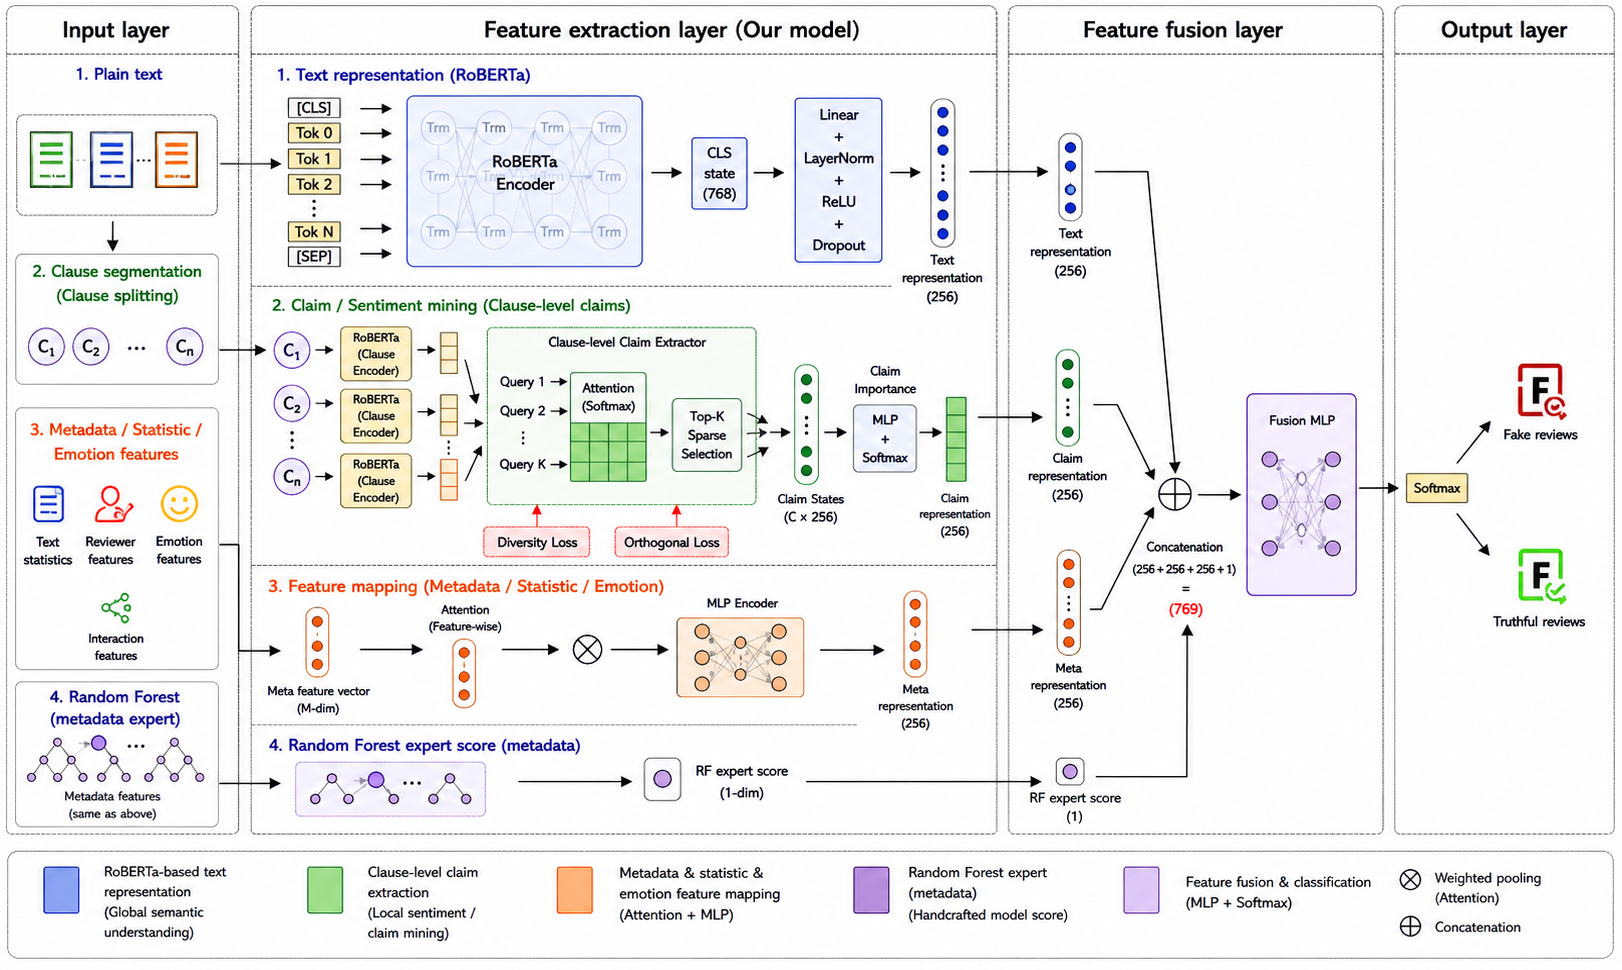
\includegraphics[width=0.95\textwidth]{figures/framework_overall.png}
  }{
    \fbox{\rule{0pt}{5cm}\rule{0.9\textwidth}{0pt}}
  }
  \caption{本文虚假餐厅评论检测模型总体框架示意图}
  \label{fig:framework}
\end{figure}

图~\ref{fig:framework} 中，上部展示了原始评论样本的来源及其标签形式，中部展示了文本预处理与元数据特征构建过程，下部展示了模型的多分支融合判别流程。与参考论文中将评论文本、情感特征与统计特征分别送入不同分支后再融合的方式类似，本文同样采用了多源信息协同建模的思路，但将“局部可疑证据建模”置于更核心的位置。

\section{输入表示与预处理}

\subsection{评论文本输入}

给定一条评论文本 $x$，首先对其进行基础清洗与编码。对于文本内容，本文保留评论原始语义信息，并采用中文预训练语言模型对应的分词器进行编码，得到输入序列
\begin{equation}
  X = [t_1,t_2,\ldots,t_L],
\end{equation}
其中 $L$ 为编码后的序列长度。编码结果包括 \texttt{input\_ids}、\texttt{attention\_mask} 以及必要时的 \texttt{token\_type\_ids}，供后续 RoBERTa 主干网络使用。

\subsection{评论分句处理}

为了增强模型对评论内部局部语义片段的感知能力，本文在输入阶段进一步对评论进行分句处理。具体地，利用中文常见标点符号“，。！？；”等对评论文本进行规则切分，得到分句集合
\begin{equation}
  x=\{c_1,c_2,\ldots,c_n\},
\end{equation}
其中 $c_i$ 表示第 $i$ 个分句。对于过长评论，本文限制最大分句数量，以控制后续计算复杂度；对于分句数不足的样本，则通过补空句的方式进行对齐，并构造相应的 \texttt{clause\_mask} 作为有效分句掩码。

这一设计的出发点在于：整条评论的整体语义表示虽然能够提供宏观判断依据，但评论中真正反映虚假性的往往是局部异常表达，如夸张性描述、模板化推销语句、细节与情绪结论不一致等。将评论切分为多个局部单元，有助于模型从更细粒度层面刻画这些异常模式。

\subsection{元数据输入}

除评论文本外，本文还使用了评论样本中可获得的结构化辅助信息。结合当前代码实现，元数据主要包括以下几类：

\begin{enumerate}
  \item 评分相关特征：如 \texttt{overall}、\texttt{taste}、\texttt{environment}、\texttt{service}、\texttt{ingredient}；
  \item 消费与展示相关特征：如 \texttt{consumption}、\texttt{food}、\texttt{picture}、\texttt{has\_picture}；
  \item 交互相关特征：如 \texttt{like}、\texttt{response}、\texttt{interaction}；
  \item 时间与统计特征：如 \texttt{publish\_hour}、\texttt{is\_weekend}、\texttt{text\_length}、\texttt{exclamation\_count}；
  \item 派生统计特征：如 \texttt{rating\_mean}、\texttt{rating\_var}、\texttt{rating\_dev}、\texttt{is\_extreme\_rating} 等。
\end{enumerate}

这些特征与参考论文中强调的 information-based 和 interaction-based 特征具有较强一致性，都是对评论文本之外的结构化辅助信息进行显式建模。参考论文通过 rich metadata 的引入提升了检测性能，并在消融实验中指出 metadata 分支贡献显著。

\section{文本全局编码模块}

对于输入评论文本，本文首先使用中文预训练语言模型 \texttt{hfl/chinese-roberta-wwm-ext} 提取全局语义表示。设输入序列经过编码后得到隐藏状态矩阵
\begin{equation}
  H=[h_1,h_2,\ldots,h_L], \quad h_i \in \mathbb{R}^{d_r},
\end{equation}
其中 $d_r$ 为 RoBERTa 隐层维度。

本文取首位特殊标记对应的表示作为评论整体语义表示，即
\begin{equation}
  h_{\mathrm{cls}} = h_1.
\end{equation}
随后通过一个线性映射层将其投影到模型内部统一的隐藏空间：
\begin{equation}
  h_g = W_c h_{\mathrm{cls}} + b_c,
\end{equation}
其中 $h_g \in \mathbb{R}^{d}$ 表示评论的全局语义表示，$d$ 为统一隐藏维度。

全局语义表示能够较好地刻画整条评论的总体内容与主观倾向，是模型进行真假判别的重要基础。但仅依赖全局表示容易将局部异常片段“平均化”，从而降低对细节证据的敏感性。因此，本文在全局语义表示之外，进一步引入细粒度评价单元抽取模块。

\section{细粒度评价单元抽取模块}

\subsection{分句级表示编码}

在获得评论的分句集合后，本文并不直接复用整条评论的 token 级表示做片段聚合，而是对每个分句单独送入同一编码器进行编码，并取各分句的全局表示作为其语义表示。设一条评论共有 $n$ 个分句，则其分句级表示记为
\begin{equation}
  U=[u_1,u_2,\ldots,u_n], \quad u_i \in \mathbb{R}^{d_r}.
\end{equation}
之后再通过线性映射与归一化层，将分句表示投影到统一隐藏空间：
\begin{equation}
  \tilde{u}_i = \mathrm{LayerNorm}(W_t u_i + b_t).
\end{equation}
由此得到分句级表示矩阵
\begin{equation}
  C=[\tilde{u}_1,\tilde{u}_2,\ldots,\tilde{u}_n], \quad \tilde{u}_i \in \mathbb{R}^{d}.
\end{equation}

\subsection{多查询评价单元抽取}

为了从多个局部语义片段中提取不同的评价关注点，本文设计了可学习查询向量集合
\begin{equation}
  Q=[q_1,q_2,\ldots,q_K], \quad q_k \in \mathbb{R}^{d},
\end{equation}
其中 $K$ 表示评价单元个数。在实现中，本文默认设置 $K=4$。

对每个查询向量，模型计算其与所有分句表示之间的匹配分数。设经过线性映射后的键向量与值向量分别为
\begin{equation}
  K_c = W_k C, \qquad V_c = W_v C,
\end{equation}
则第 $k$ 个查询向量对应的注意力分数可表示为
\begin{equation}
  s_{k,i} = \frac{q_k^\top k_i}{\sqrt{d}},
\end{equation}
其中 $k_i$ 表示第 $i$ 个分句对应的键向量。结合分句掩码后，经 softmax 归一化得到注意力权重：
\begin{equation}
  \alpha_{k,i} = \mathrm{softmax}(s_{k,i}).
\end{equation}
最终，第 $k$ 个评价单元表示为
\begin{equation}
  z_k = \sum_{i=1}^{n} \alpha_{k,i} v_i,
\end{equation}
其中 $v_i$ 表示第 $i$ 个分句对应的值向量。

通过这一机制，不同查询向量能够分别关注评论内部不同的语义片段，使模型具备从局部层面抽取多种判别证据的能力。与参考论文中用独立 TextCNN 分支显式建模情感特征不同，本文将更多建模能力投入到评论内部局部证据的提取上，以突出“哪一部分内容更可疑”这一任务目标。

\subsection{细粒度评价单元对虚假评论检测的作用}

在虚假评论检测任务中，评论是否虚假往往并不由整段文本的单一情感倾向决定，而是隐藏在若干局部表达模式中。真实评论通常包含较具体的消费过程、对象细节和正负混合体验，例如到店背景、菜品名称、服务细节、价格或规则争议等；而虚假评论更容易出现模板化推荐、过度堆叠的情绪词、缺少具体经历支撑的笼统评价，或者评分结论与文本证据不一致等现象。如果只使用整条评论的 \texttt{[CLS]} 向量，模型会将这些局部片段压缩为一个全局表示，容易使关键异常线索被大量普通描述“平均化”。

细粒度评价单元的作用正是把整条评论拆解为若干可被单独关注的局部证据。具体而言，多个 Claim 查询可以分别承担不同的观察角度：有的 Claim 关注消费场景和事实性细节，有的 Claim 关注情绪结论或推荐意向，有的 Claim 关注服务、价格、菜品等具体评价维度，还有的 Claim 关注反问、夸张、重复等表达模式。这样，模型在判断评论真假时不再只回答“整段评论整体像不像虚假评论”，而是进一步判断“哪些局部片段支持真实体验，哪些局部片段表现出可疑模式”。

从检测逻辑上看，细粒度评价单元主要通过三种方式支持虚假评论检测。第一，它增强了局部异常感知能力，使模型能够捕捉模板化、夸张化或空泛化表达；第二，它保留了多维度证据结构，使模型能够区分“真实评论中的负面投诉”和“缺少细节支撑的负面攻击”；第三，它提供了可解释的注意力分布，使最终判断能够回溯到具体分句或局部片段。表~\ref{tab:claim-detection-role} 总结了细粒度评价单元与虚假评论检测信号之间的对应关系。

\begin{table}[htbp]
  \centering
  \small
  \caption{细粒度评价单元支持虚假评论检测的主要方式}
  \label{tab:claim-detection-role}
  \begin{tabularx}{\textwidth}{lXX}
    \toprule
    建模角度 & 可能捕捉的局部内容 & 对虚假评论检测的作用 \\
    \midrule
    消费过程细节 & 到店背景、点餐内容、服务过程、具体问题 & 判断评论是否具有真实体验支撑，减少仅凭情绪词误判。 \\
    情绪与推荐意向 & 强烈推荐、强烈否定、反问、总结性态度 & 捕捉评论的总体立场和可能的夸张表达。 \\
    维度化评价 & 菜品、环境、服务、价格、规则等局部评价 & 区分评论是否围绕具体对象展开，而不是泛泛而谈。 \\
    一致性关系 & 评分与文本、正向细节与负向结论之间的关系 & 发现情绪结论与细节证据不匹配的可疑模式。 \\
    模板化表达 & 高频宣传语、重复推荐词、缺少对象细节的套话 & 辅助识别刷评或生成式评论中常见的模式化语言。 \\
    \bottomrule
  \end{tabularx}
\end{table}

\subsection{评价单元重要性聚合}

在得到多个评价单元表示后，本文进一步使用一个重要性估计网络为各评价单元分配权重。具体而言，先对每个评价单元表示 $z_k$ 计算其重要性得分：
\begin{equation}
  \gamma_k = W_s z_k + b_s,
\end{equation}
随后通过 softmax 归一化：
\begin{equation}
  \beta_k = \frac{\exp(\gamma_k)}{\sum_{j=1}^{K}\exp(\gamma_j)}.
\end{equation}
据此可得到综合评价单元表示
\begin{equation}
  h_c = \sum_{k=1}^{K} \beta_k z_k.
\end{equation}

这一聚合过程的作用在于：不同评价单元虽然分别关注评论中的不同局部片段，但它们对最终真假判别的贡献并不相同。通过显式学习评价单元重要性，模型能够在保持多视角局部建模能力的同时，进一步提炼出最具判别价值的局部证据表示。

\subsection{评价单元门控融合}

考虑到局部证据分支过强可能会对整体语义判断造成干扰，本文在全局文本表示与评价单元表示之间引入门控机制。具体地，将全局表示 $h_g$ 与综合评价单元表示 $h_c$ 拼接后输入门控网络：
\begin{equation}
  g = \sigma(W_g[h_g;h_c]+b_g),
\end{equation}
其中 $g \in (0,1)$ 表示门控系数。随后，对评价单元表示进行平滑缩放：
\begin{equation}
  h_c^{\prime} = h_c \cdot (0.25 + 0.50g).
\end{equation}

与直接令局部证据分支等权参与融合相比，这种平滑门控机制能够根据样本内容动态控制评价单元分支的影响程度，使其既能提供局部异常感知能力，又不会过度破坏全局语义的稳定性。

\section{元数据辅助分支}

参考已有元数据感知虚假评论检测研究，本文同样将评论元数据视为重要的判别信息来源。不同于将所有结构化特征直接与文本向量拼接，本文首先通过注意力机制对元数据各维度进行动态加权，再通过多层感知机学习其高层表示。

设原始元数据向量为
\begin{equation}
  m=[m_1,m_2,\ldots,m_p].
\end{equation}
在输入模型前，先对连续特征进行标准化处理，得到 $\tilde{m}$。随后利用元数据注意力网络计算各维度权重：
\begin{equation}
  a_m = \sigma(W_a \tilde{m} + b_a),
\end{equation}
并对原始特征逐元素加权：
\begin{equation}
  \tilde{m}^{\,\prime} = a_m \odot \tilde{m}.
\end{equation}
在此基础上，将加权后的元数据输入多层感知机，得到高层表示
\begin{equation}
  h_m = \mathrm{MLP}(\tilde{m}^{\,\prime}).
\end{equation}

从功能上看，元数据分支主要负责从评分模式、交互统计、展示信息和时间分布等角度补充结构化判别线索。结合你当前的实验结果，这一分支对整体性能提升具有重要作用，也与参考论文中“metadata contributes greatly”这一结论一致。

\section{随机森林元数据专家分数模块}

除神经网络中的元数据辅助分支外，本文还引入基于随机森林的元数据专家分数，以补充另一种结构化判别视角。随机森林是一种典型的集成学习方法，适合处理元数据中的非线性组合关系。设输入的标准化元数据为 $\tilde{m}$，随机森林输出该评论属于虚假评论的概率为
\begin{equation}
  s_{\mathrm{rf}} = g(\tilde{m}),
\end{equation}
其中 $g(\cdot)$ 表示随机森林分类器。

在训练过程中，为避免信息泄漏，本文对训练集采用基于内层交叉验证的 out-of-fold 方式生成训练样本上的专家分数；对验证集则使用基于完整训练集拟合的随机森林模型进行打分。最终，一维专家分数 $s_{\mathrm{rf}}$ 与深度模型输出的其他表示共同参与融合分类。

这一设计的意义在于：深度模型擅长从文本与元数据中学习连续高维表示，而随机森林更擅长利用结构化特征中的树型分裂关系与非线性组合模式。将两者结合，有助于提升模型对复杂虚假评论模式的综合识别能力。

\section{特征融合与分类输出}

在获得全局文本表示、细粒度评价单元表示、元数据高层表示以及随机森林专家分数后，本文将它们进行联合融合。具体地，最终融合特征写为
\begin{equation}
  h_f = [h_g;h_c^{\prime};h_m;s_{\mathrm{rf}}],
\end{equation}
其中 $[\cdot;\cdot]$ 表示向量拼接。

随后，将融合表示输入全连接分类器，得到二分类 logits：
\begin{equation}
  o = W_f h_f + b_f.
\end{equation}
在二分类场景下，评论属于虚假评论的预测概率可写为
\begin{equation}
  \hat{y} = \mathrm{softmax}(o).
\end{equation}

从整体上看，该融合机制实现了多源信息的协同利用：全局文本表示负责提供评论整体语义背景，评价单元分支负责强调局部异常片段，元数据分支负责提供结构化辅助判断，而随机森林专家分数则补充另一种机器学习视角下的元数据先验判断。

\section{损失函数与训练策略}

\subsection{分类损失}

本文采用交叉熵损失作为基本分类目标。设真实标签为 $y$，预测概率为 $\hat{y}$，则分类损失为
\begin{equation}
  \mathcal{L}_{\mathrm{cls}} = - \sum_{c=1}^{C} y_c \log \hat{y}_c,
\end{equation}
其中 $C=2$ 表示类别数。

\subsection{评价单元多样性约束}

为避免不同评价单元重复关注相同的分句区域，本文在训练过程中进一步引入评价单元多样性损失。设评价单元注意力矩阵为 $A\in\mathbb{R}^{K\times n}$，则通过约束不同评价单元注意力分布之间的重叠程度，得到多样性损失项
\begin{equation}
  \mathcal{L}_{\mathrm{div}} = \mathrm{Overlap}(A).
\end{equation}
最终总损失写为
\begin{equation}
  \mathcal{L} = \mathcal{L}_{\mathrm{cls}} + \lambda \mathcal{L}_{\mathrm{div}},
\end{equation}
其中 $\lambda$ 为多样性损失权重。

该正则项的作用在于鼓励不同评价单元关注评论中的不同局部片段，从而增强细粒度建模的区分性与可解释性。

\subsection{两阶段训练策略}

在优化策略上，本文采用两阶段训练方式。第一阶段冻结 RoBERTa 编码器，仅训练新增的评价单元分支、元数据辅助分支及分类器，以使新增模块先获得较稳定初始化；第二阶段解冻编码器，进行全模型联合训练，从而进一步提升整体检测性能。

同时，本文对预训练编码器与新增模块采用分层学习率设置：RoBERTa 编码器使用较小学习率，而评价单元分支、元数据分支和分类头使用较大学习率。这一策略有助于在保持预训练知识稳定性的同时，提高下游任务适配效率。参考论文也采用了冻结部分预训练模块、动态优化与早停等策略以提升训练稳定性。

\section{模型实现细节}

本文模型基于 PyTorch 与 HuggingFace Transformers 框架实现，文本主干编码器使用 \texttt{hfl/\allowbreak chinese-\allowbreak roberta-\allowbreak wwm-\allowbreak ext}。在数据处理阶段，评论文本经分词器编码后生成 \texttt{input\_ids}、\texttt{attention\_mask} 等输入；分句结果通过自定义 \texttt{Dataset} 与 \texttt{collator} 组织成统一批次，同时构造 \texttt{clause\_mask} 以标识有效分句位置。

在元数据处理方面，首先完成固定字段提取与派生统计特征构建，然后通过标准化方法统一量纲，再输入元数据辅助分支与随机森林元数据专家分数模块。为缓解类别不平衡带来的训练偏置，本文在实验设置中结合 NearMiss-1 欠采样和分层十折交叉验证对模型进行系统评估。

需要说明的是，正文部分主要介绍模型功能结构、关键设计思想与训练逻辑，关键源码实现请在附录中查看。
% ==================================================
% 第4章 实验设计与结果分析
% ==================================================
\chapter{实验设计与结果分析}

\section{数据集与预处理}
本文实验使用大众点评虚假餐厅评论数据集中的 Dp-TDC 数据作为主实验数据。该数据来自大众点评平台，包含评论文本、真假标签以及评分、会员、折扣、图片、点赞、商家回复、互动次数、发布时间等元数据字段。标签中，$1$ 表示虚假评论，$0$ 表示真实评论。

根据数据文件统计，本文主实验共使用 32004 条大众点评评论，其中真实评论 26988 条，虚假评论 5016 条。表~\ref{tab:dataset} 给出了本文实验所用数据的基本统计信息。

\begin{table}[htbp]
  \centering
  \caption{大众点评主实验数据统计}
  \label{tab:dataset}
  \begin{tabular}{lcccc}
    \toprule
    数据集 & 领域 & 样本数 & 真实评论 & 虚假评论 \\
    \midrule
    Dp-TDC & 餐饮评论 & 32004 & 26988 & 5016 \\
    \bottomrule
  \end{tabular}
\end{table}

图~\ref{fig:data-processing-flow} 概括了本文从大众点评原始评论到模型输入构造的整体处理流程。原始样本同时包含评论文本、真假标签和平台元数据；经过文本分句、字段清洗、派生特征构建和元数据向量化后，最终形成由全文文本、细粒度分句片段和结构化元数据共同组成的模型输入。

\begin{figure}[htbp]
  \centering
  \IfFileExists{figures/data_processing_flow.png}{
    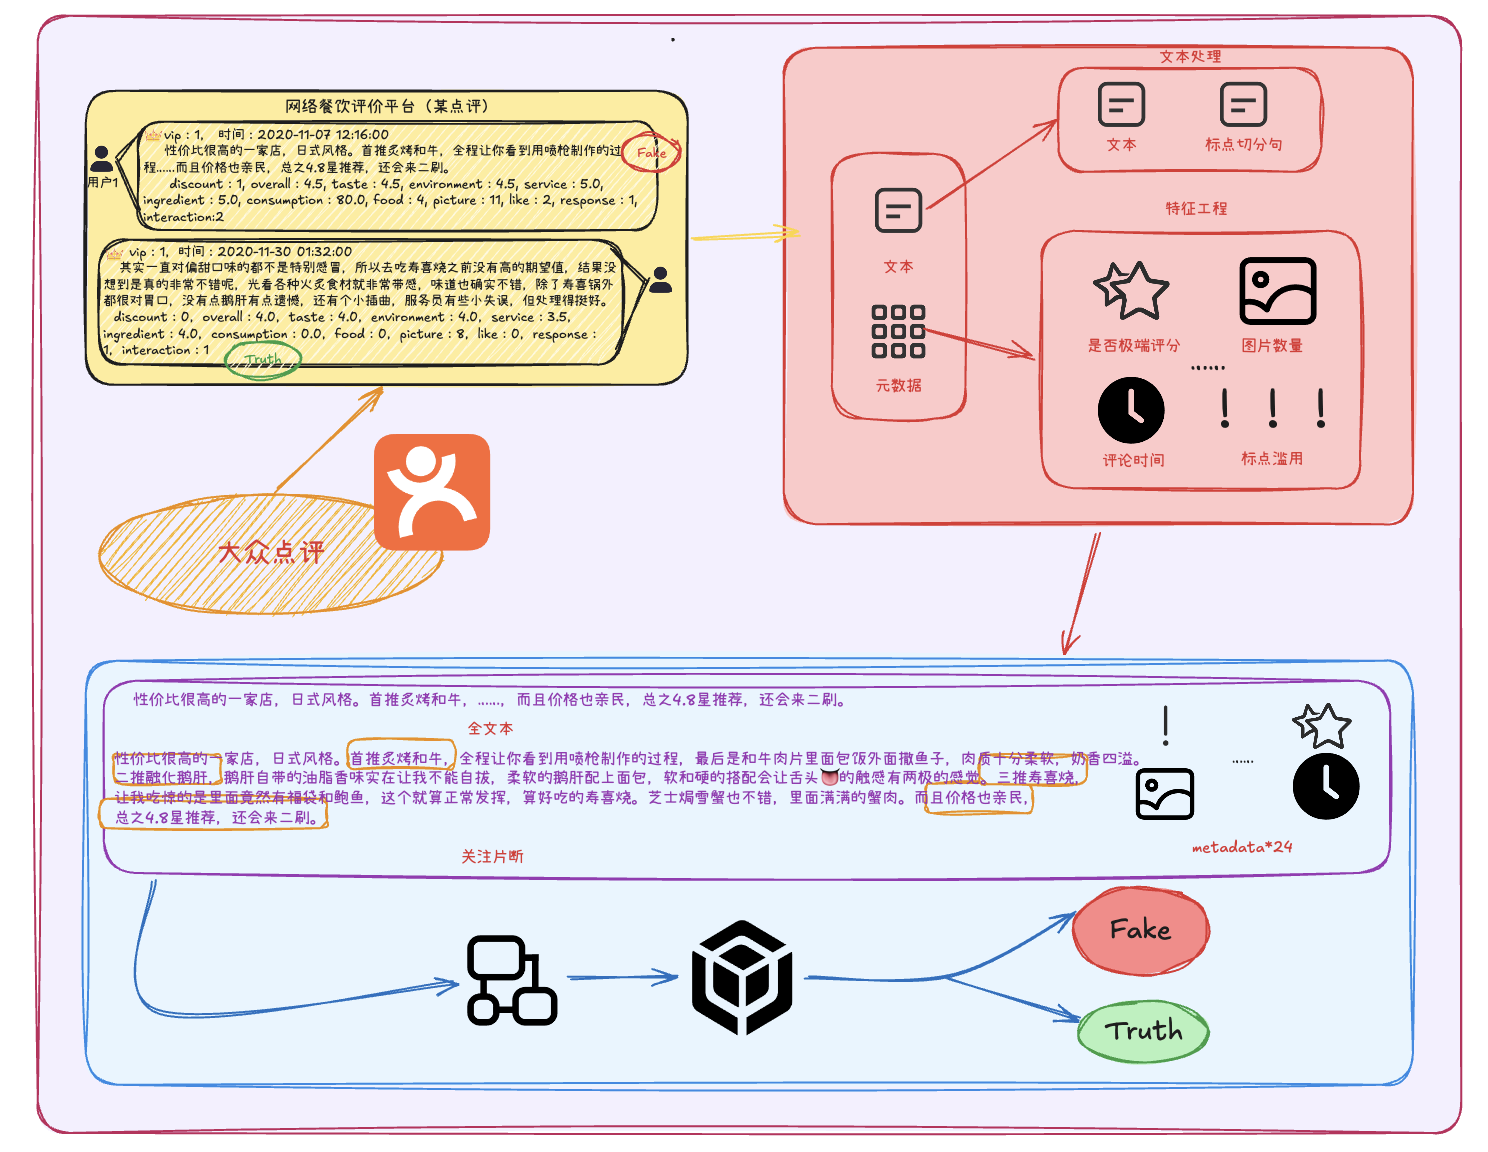
\includegraphics[width=0.95\textwidth]{figures/data_processing_flow.png}
  }{
    \fbox{\rule{0pt}{6.0cm}\rule{0.95\textwidth}{0pt}}
  }
  \caption{大众点评评论数据处理与模型输入构造流程}
  \label{fig:data-processing-flow}
\end{figure}

在预处理阶段，本文首先对原始数据字段进行统一检查与类型转换。对于输入数据，要求至少包含评论文本字段 \texttt{text} 与标签字段 \texttt{label}，并将标签统一转换为整数形式，用于后续二分类训练。若数据中存在城市相关字段，如 \texttt{city}、\texttt{shop\_city}、\texttt{region} 或 \texttt{district\_city}，则优先保留该字段作为城市分组依据；若不存在有效城市字段，则统一构造 \texttt{city=GLOBAL}，使后续 NearMiss-1 采样能够退化为全局欠采样。此处设计是为以后能够爬取到大众点评的新数据而设计，在本项目中的数据集由于安全需要没有公开店铺名称、位置、用户ID，因此店铺区域均使用统一标识，未起到作用；对于元数据中可能缺失的基础数值字段，如会员标识、折扣、总体评分、口味评分、环境评分、服务评分、食材评分、消费金额、推荐菜数量、图片数量、点赞数、商家回复和互动数等，本文统一补充默认值 0，并将其转换为数值类型，以避免字段缺失导致模型输入维度不一致。

在文本处理方面，本文将评论内容统一转换为字符串形式，并基于中文和英文常见标点符号对评论进行分句切分。具体而言，使用“，。！？；;,.!?”等符号作为切分边界，将一条评论划分为若干局部片段；若切分后不存在有效片段，则保留原始评论文本作为唯一分句。为控制计算复杂度，每条评论最多保留前 16 个分句，并将分句结果存入 \texttt{clauses} 字段，供后续细粒度评价单元抽取模块使用。与此同时，文本部分仍使用中文 RoBERTa 分词器进行编码，并统一截断或填充到固定长度，生成模型所需的 \texttt{input\_ids}、\texttt{attention\_mask} 等输入。

在时间和文本统计特征构建方面，本文将 \texttt{time} 字段转换为时间类型，并进一步提取评论发布时间小时 \texttt{publish\_hour}、是否周末 \texttt{is\_weekend} 以及是否处于正常发布时间段 \texttt{valid\_post\allowbreak\_hour}。其中，\texttt{valid\_post\_hour} 用于刻画评论是否发布于 6:00 至 23:00 之间。对于文本形态，本文构造评论长度 \texttt{text\_length}、感叹号与问号数量 \texttt{exclamation\_count} 等统计特征，以反映评论表达强度和文本复杂度。

在评分与展示特征构建方面，本文根据图片数量生成是否含图片特征 \texttt{has\_picture}，根据消费金额生成是否存在消费金额特征 \texttt{has\_consumption}，并基于总体评分构造是否极端评分特征 \texttt{is\_extreme\_rating}。同时，本文进一步计算口味、环境、服务和食材等子评分的均值 \texttt{rating\_mean}，以及总体评分与各子评分之间的方差 \texttt{rating\_var} 和偏差 \texttt{rating\_dev}，用于刻画评分内部的一致性与异常程度。

最终，本文将原始元数据与派生统计特征共同组成固定维度的元数据向量。该向量共包含 24 个特征，包括用户与优惠信息、评分信息、消费与展示信息、交互信息、时间信息、文本统计信息以及评分一致性特征。所有元数据特征在输入模型前均转换为数值类型并填充缺失值，保证后续元数据分支、随机森林专家分数模块和 NearMiss-1 采样过程能够使用统一的特征空间。图~\ref{fig:featuregroup} 给出了本文使用的主要特征类别。

\begin{figure}[htbp]
  \centering
  \begin{tikzpicture}[
    font=\songti\zihao{5},
    category/.style={
      draw=black!55,
      fill=blue!9,
      rounded corners=2pt,
      minimum width=3.0cm,
      minimum height=0.82cm,
      align=center
    },
    feature/.style={
      draw=black!35,
      fill=gray!7,
      rounded corners=2pt,
      minimum height=0.82cm,
      text width=9.0cm,
      align=left,
      inner xsep=8pt
    },
    link/.style={draw=black!45, line width=0.45pt}
  ]
    \node[category] (c1) {用户与优惠特征};
    \node[feature, right=0.45cm of c1] (f1) {\texttt{vip}、\texttt{discount}};

    \node[category, below=0.34cm of c1] (c2) {评分特征};
    \node[feature, right=0.45cm of c2] (f2) {\texttt{overall}、\texttt{taste}、\texttt{environment}、\texttt{service}、\texttt{ingredient}、\texttt{is\_extreme\_rating}};

    \node[category, below=0.34cm of c2] (c3) {内容形态特征};
    \node[feature, right=0.45cm of c3] (f3) {\texttt{picture}、\texttt{has\_picture}、\texttt{text\_length}、\texttt{exclamation\_count}};

    \node[category, below=0.34cm of c3] (c4) {交互特征};
    \node[feature, right=0.45cm of c4] (f4) {\texttt{like}、\texttt{response}、\texttt{interaction}};

    \node[category, below=0.34cm of c4] (c5) {时间特征};
    \node[feature, right=0.45cm of c5] (f5) {\texttt{publish\_hour}、\texttt{is\_weekend}};

    \foreach \i in {1,...,5} {
      \draw[link] (c\i.east) -- (f\i.west);
    }
  \end{tikzpicture}
  \caption{元数据与派生特征类别}
  \label{fig:featuregroup}
\end{figure}

\begin{figure}[htbp]
  \centering
  \IfFileExists{figures/dataset_label_distribution.png}{
    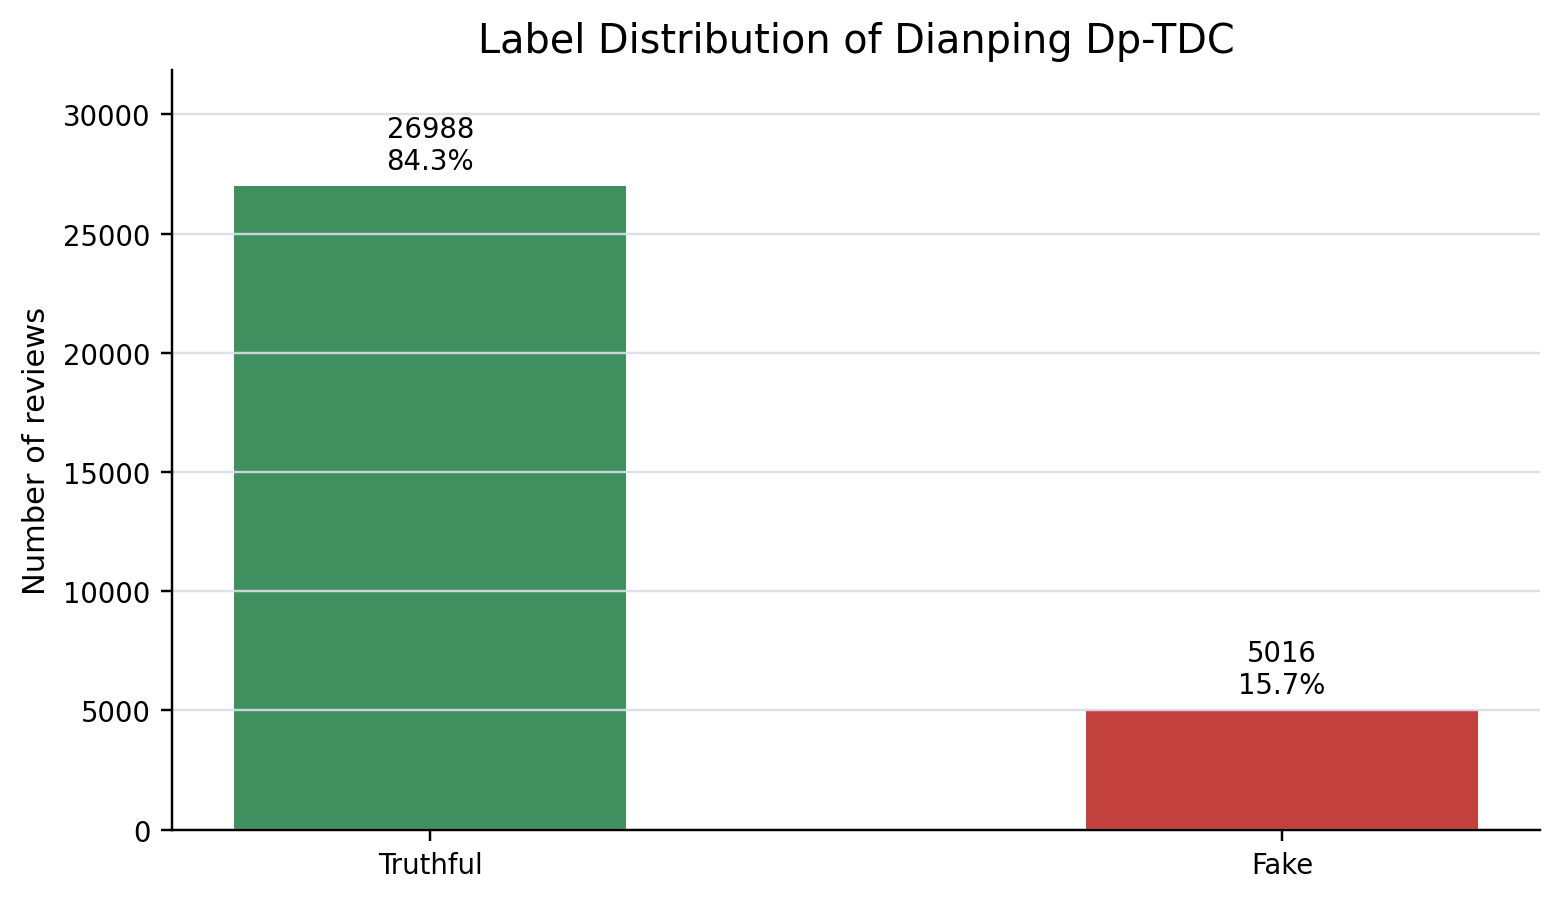
\includegraphics[width=0.72\textwidth]{figures/dataset_label_distribution.png}
  }{
    \fbox{\rule{0pt}{4.6cm}\rule{0.72\textwidth}{0pt}}
  }
  \caption{大众点评数据标签分布}
  \label{fig:dataset-label-distribution}
\end{figure}

\section{实验环境与参数设置}
本文实验在本地 macOS 环境和 Linux 服务器环境下完成。其中，macOS 主要用于数据预处理、特征检查、模型原型调试和结果整理；Linux 服务器我只能使用一张 NVIDIA RTX 3090 GPU，主要用于 RoBERTa、Claim 模型及融合模型的训练与十折交叉验证。表~\ref{tab:env} 给出了实验环境设置。

\begin{table}[htbp]
  \centering
  \caption{实验环境设置}
  \label{tab:env}
  \begin{tabular}{ll}
    \toprule
    项目 & 设置 \\
    \midrule
    本地调试环境 & macOS \\
    服务器训练环境 & Linux，NVIDIA RTX 3090 GPU \\
    编程语言 & Python 3.10 \\
    深度学习框架 & PyTorch、HuggingFace Transformers \\
    机器学习工具 & scikit-learn、imbalanced-learn \\
    预训练模型 & \texttt{hfl/chinese-roberta-wwm-ext} \\
    \bottomrule
  \end{tabular}
\end{table}

表~\ref{tab:hyper} 给出了主要模型训练参数。纯文本 RoBERTa 和 Claim 系列模型均采用最大长度 128 的输入设置；两阶段训练时，第一阶段冻结 RoBERTa，仅训练新增模块，第二阶段解冻 RoBERTa 并进行联合微调。

\begin{table}[htbp]
  \centering
  \caption{模型主要参数设置}
  \label{tab:hyper}
  \begin{tabular}{lll}
    \toprule
    参数 & 取值 & 说明 \\
    \midrule
    max\_length & 128 & 文本最大长度 \\
    train batch size & 8 & RoBERTa/Claim 训练批大小 \\
    eval batch size & 16 & 验证批大小 \\
    learning rate & $2\times10^{-5}$ & 主干联合微调学习率 \\
    stage-1 learning rate & $1\times10^{-4}$ & 冻结 RoBERTa 时新增模块学习率 \\
    epochs & 3 & 常规微调轮数 \\
    num\_claims & 4 或 6 & 评价单元查询个数 \\
    hidden\_dim & 256 & Claim 分支隐层维度 \\
    dropout & 0.1 & Dropout 比例 \\
    \bottomrule
  \end{tabular}
\end{table}

\section{基线模型对比实验}
为验证不同信息来源对虚假评论检测的贡献，本文首先设置三类基线：仅使用结构化元数据的随机森林模型、仅使用评论文本的 RoBERTa 模型，以及融合文本、细粒度评价单元、元数据分支和随机森林专家分数的完整模型。表~\ref{tab:baseline} 给出了主要基线与最终模型的对比结果。

\begin{table}[htbp]
  \centering
  \caption{基线模型与最终模型对比}
  \label{tab:baseline}
  \resizebox{\textwidth}{!}{
  \begin{tabular}{lccccc}
    \toprule
    模型 & 信息来源 & Accuracy & Precision & Recall & F1 \\
    \midrule
    随机森林 & Metadata & 0.8833 & 0.6400 & 0.5900 & 0.6100 \\
    RoBERTa & Text & 0.8400 & 0.8361 & 0.8182 & 0.8270 \\
    Claim+Metadata+RF & Text+Claim+Metadata+RF & 0.9272 & 0.9340 & 0.9199 & 0.9266 \\
    Claim+Metadata+RF（最佳阈值） & Text+Claim+Metadata+RF & 0.9276 & 0.9191 & 0.9378 & 0.9284 \\
    \bottomrule
  \end{tabular}}
\end{table}

从表~\ref{tab:baseline} 可以看出，随机森林仅依赖元数据即可取得 0.8833 的 Accuracy，说明结构化行为特征在大众点评虚假评论检测中具有较强区分能力。纯文本 RoBERTa 的 F1 为 0.8270，说明文本语义能够提供较稳定的判别信息。最终融合模型在十折交叉验证下取得 0.9272 的 Accuracy 和 0.9266 的 F1，显著优于单一信息来源模型；经过阈值搜索后，Recall 提升至 0.9378，F1 进一步达到 0.9284。

\begin{figure}[htbp]
  \centering
  \IfFileExists{figures/baseline_comparison.png}{
    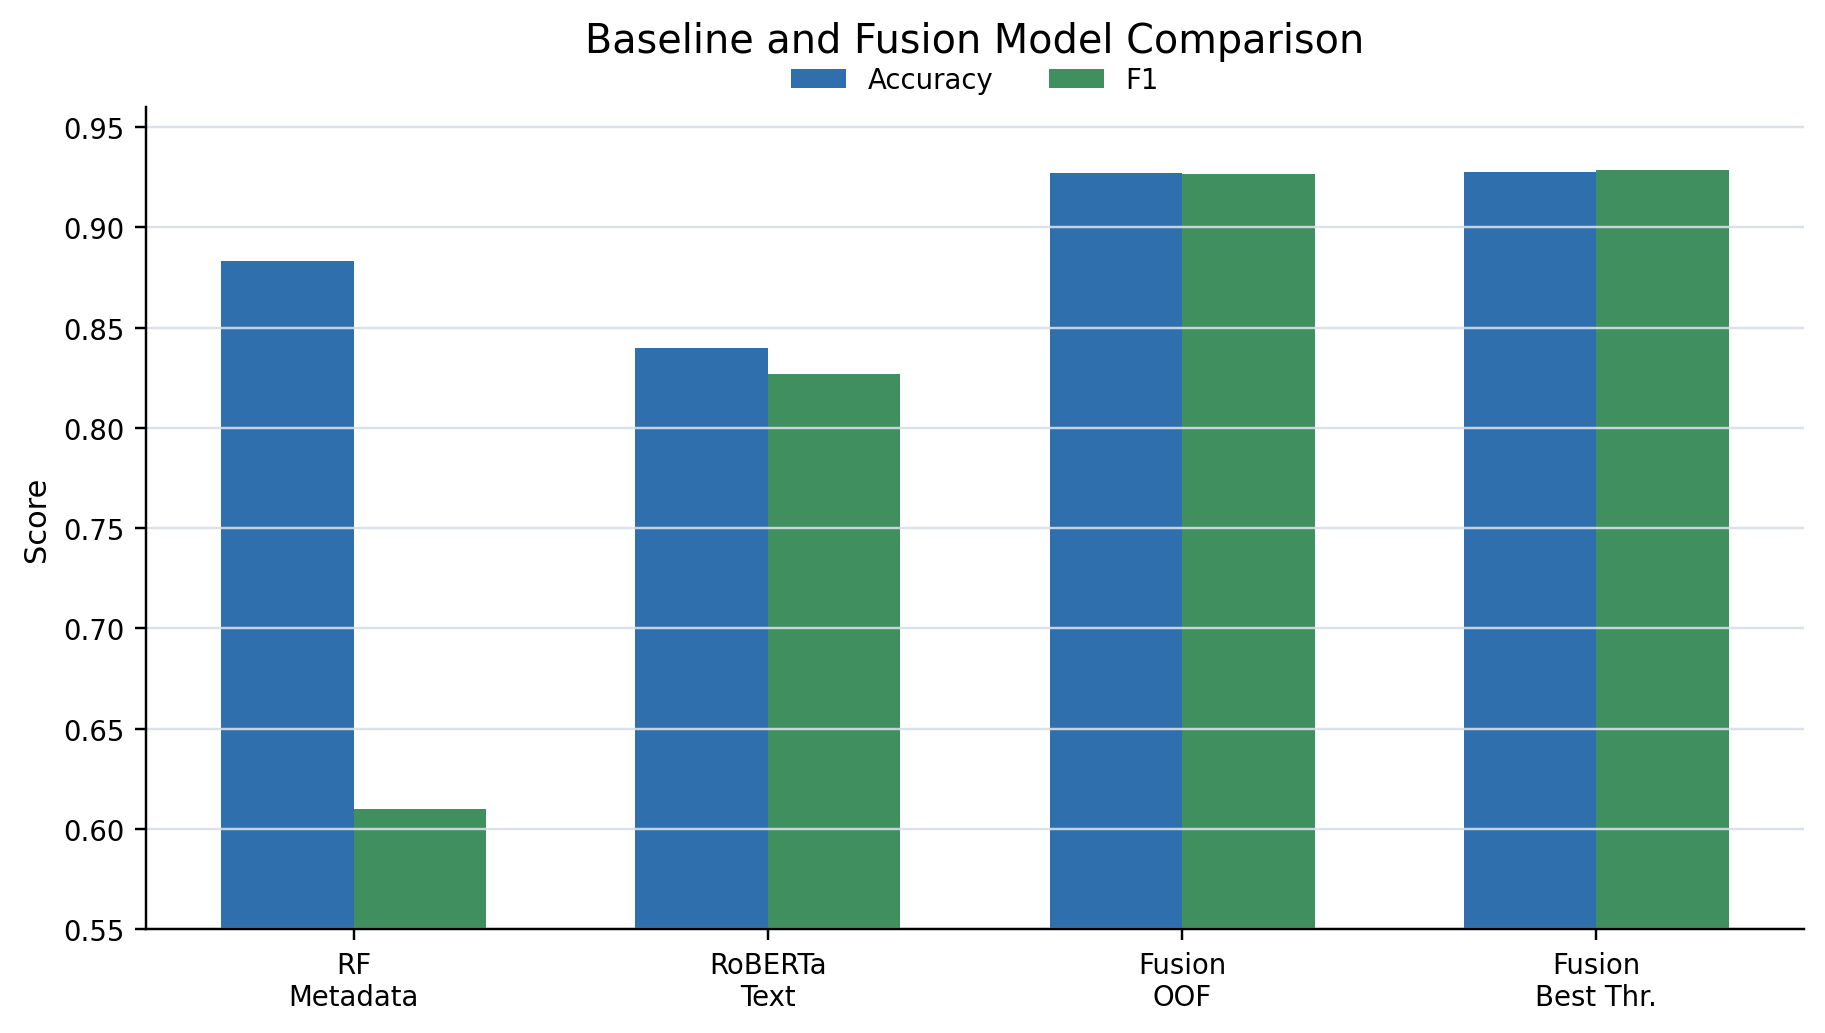
\includegraphics[width=0.82\textwidth]{figures/baseline_comparison.png}
  }{
    \fbox{\rule{0pt}{5.0cm}\rule{0.82\textwidth}{0pt}}
  }
  \caption{基线模型与最终模型性能对比}
  \label{fig:baseline-comparison}
\end{figure}

\section{细粒度评价单元建模实验}
为分析细粒度评价单元分支的有效性，本文围绕 Claim 模块进行了多组中间实验。这些实验并不是最终模型的完整形态，而是用于回答三个问题：第一，仅在文本分支中引入多个可学习评价单元是否有效；第二，多个评价单元之间是否需要多样性约束；第三，训练策略和评价单元聚合方式会不会影响模型表现。

本文所称 Claim 分支，是指在 RoBERTa 编码结果之上，将评论文本切分为若干分句或局部片段，再通过多个可学习查询向量从局部表示中抽取若干细粒度评价单元。每个评价单元可理解为模型从评论中主动寻找的一类局部证据，例如消费过程描述、情绪评价、推荐理由、夸张表达或模板化表述等。相比只使用 \texttt{[CLS]} 全局向量，Claim 分支希望让模型显式关注评论内部的局部可疑线索。

对于虚假评论检测而言，这种细粒度建模的意义主要体现在“证据定位”和“证据组合”两个方面。证据定位是指模型能够从长评论中找出更值得关注的局部片段，例如服务投诉、规则争议、反问式总结、模板化推荐语等；证据组合是指模型不会孤立地依据某一个情绪词进行判断，而是综合多个评价单元形成最终表示。例如，一条真实差评可能同时包含具体消费过程、菜品正向细节和服务负向细节；如果模型只看到“态度恶劣”等负向词，容易将其误判为攻击性虚假评论，而 Claim 分支可以同时保留“具体到店背景”“菜品细节”“投诉对象”等局部证据，从而帮助模型判断该评论是否具有真实体验支撑。

因此，本节的 Claim 实验并不只用于追求单独分类指标，而是用于验证细粒度评价单元能否形成有效的局部证据表示。小样本实验重点观察 diversity loss 是否能让不同 Claim 覆盖不同片段；全量实验重点观察训练策略和聚合方式是否能稳定提取这些局部证据。后续融合模型再将 Claim 表示与元数据分支结合，使文本内部证据与行为结构证据共同参与虚假评论检测。

表~\ref{tab:claim-setting} 对本节涉及的几个实验变量进行说明。其中，一阶段和两阶段属于训练策略差异，mean-max 属于评价单元聚合方式差异，diversity loss 属于损失函数层面的约束。

\begin{table}[htbp]
  \centering
  \caption{Claim 实验变量说明}
  \label{tab:claim-setting}
  \begin{tabularx}{\textwidth}{lX}
    \toprule
    实验变量 & 含义与作用 \\
    \midrule
    一阶段训练 & 直接解冻 RoBERTa，并与 Claim 分支、分类器一起端到端联合训练。 \\
    两阶段训练 & 第一阶段冻结 RoBERTa，仅训练 Claim 分支和分类器；第二阶段解冻 RoBERTa 进行联合微调。 \\
    mean-max 聚合 & 对多个 Claim 表示同时计算平均池化和最大池化，再拼接形成评论级 Claim 表示。 \\
    无 mean-max 聚合 & 使用注意力加权或门控方式汇总 Claim 表示，不额外拼接最大池化统计。 \\
    diversity loss & 约束不同 Claim 查询关注不同局部片段，减少多个评价单元学到重复信息。 \\
    \bottomrule
  \end{tabularx}
\end{table}

从训练稳定性的角度看，一阶段训练实现简单，但新增的 Claim 分支参数随机初始化，容易在训练初期对 RoBERTa 主干产生较大梯度扰动。两阶段训练的改进在于，先固定预训练主干，让新增的 Claim 分支和分类器先学习较稳定的任务相关表示；随后再解冻 RoBERTa，使全模型联合适配虚假评论检测任务。因此，两阶段训练更适合“预训练主干 + 新增结构模块”的设置。

从特征聚合的角度看，早期实验主要比较了 mean pooling 与 mean-max 聚合两类策略。mean pooling 是对多个评价单元表示进行简单平均，其形式可写为 $h_c=\frac{1}{K}\sum_{k=1}^{K}z_k$。该方法实现简单、训练稳定，能够反映多个评价单元的整体平均语义，但其缺点也较明显：所有 Claim 被赋予相同权重，模型无法区分哪些局部证据更关键，容易将强判别片段与普通片段一起平均，从而削弱局部异常信号。mean-max 聚合则在平均池化之外进一步引入最大池化，即同时保留多个评价单元的整体趋势和局部峰值信号。理论上，max pooling 能突出某个 Claim 上最强的可疑信息；但在实际实验中，最大池化也容易放大个别强情绪词、功能词或非关键分句带来的噪声，尤其当评论较长、分句数量较多时，这类噪声会影响最终表示的稳定性。因此，本文将 mean-max 作为候选聚合策略进行验证，而没有直接作为最终方案。

当前源码中的最终模型并未采用简单 mean pooling，也未采用 mean-max 拼接，而是采用“Claim 重要性加权聚合 + 门控融合”的方式。具体而言，模型先通过一个重要性估计网络为每个评价单元 $z_k$ 计算权重 $\beta_k$，再得到加权综合表示 $h_c=\sum_{k=1}^{K}\beta_k z_k$；随后再利用门控系数控制 Claim 表示对全局文本表示的影响强度。与 mean pooling 相比，该方法能够根据样本内容动态突出更有判别力的评价单元，而不是对所有 Claim 等权平均；与 mean-max 聚合相比，该方法不会直接取最大响应，因此能够降低单个噪声片段或极端词语被过度放大的风险。同时，门控机制还能在 Claim 分支不稳定时自动降低其影响，使局部证据作为全局 RoBERTa 表示的补充信息参与融合。因而，当前源码采用的加权门控聚合方式在稳定性、可解释性和局部证据利用之间取得了更好的平衡。

\begin{table}[htbp]
  \centering
  \caption{小样本 Claim 损失函数对比}
  \label{tab:claim-small}
  \begin{tabular}{lccccc}
    \toprule
    模型设置 & 数据规模 & Accuracy & Precision & Recall & F1 \\
    \midrule
    cls\_loss & 1000 & 0.8225 & 0.8021 & 0.8235 & 0.8127 \\
    cls\_loss+diversity\_loss & 1000 & 0.8325 & 0.8158 & 0.8289 & 0.8223 \\
    \bottomrule
  \end{tabular}
\end{table}

表~\ref{tab:claim-small} 表明，在 1000 条样本设置下，加入 diversity loss 后 Accuracy 从 0.8225 提升至 0.8325，F1 从 0.8127 提升至 0.8223。这说明多个 Claim 查询如果只依赖分类损失，可能会集中关注相似的高频表达；加入多样性约束后，不同评价单元能够覆盖更多局部证据，从而改善小样本条件下的表示质量。


\begin{table}[htbp]
  \centering
  \small
  \caption{全量数据 Claim 训练策略与聚合方式对比}
  \label{tab:claim-full}
  \begin{tabular}{lccccc}
    \toprule
    模型设置 & Accuracy & Precision & Recall & F1 & 主要差异 \\
    \midrule
    无 mean-max，一阶段 & 0.9099 & 0.7404 & 0.6748 & 0.7061 & 直接联合训练 \\
    无 mean-max，两阶段 & 0.9106 & 0.7367 & 0.6894 & 0.7123 & 先冻结后联合 \\
    mean-max，两阶段 & 0.9028 & 0.6938 & 0.7059 & 0.6998 & 改变 Claim 聚合 \\
    mean-max，一阶段 & 0.9080 & 0.7156 & 0.7079 & 0.7117 & mean-max 且无冻结 \\
    \bottomrule
  \end{tabular}
\end{table}


表~\ref{tab:claim-full} 展示了全量数据上的训练策略和聚合方式对比。首先，在不使用 mean-max 聚合时，两阶段训练的 F1 为 0.7123，高于一阶段训练的 0.7061，说明先冻结 RoBERTa、再联合微调的方式确实有助于 Claim 分支稳定学习。其次，mean-max 聚合没有稳定带来提升：两阶段 mean-max 的 F1 为 0.6998，低于无 mean-max 两阶段模型；一阶段 mean-max 的 F1 为 0.7117，虽接近两阶段模型，但 Precision 仍低于无 mean-max 两阶段设置。这表明 mean-max 虽然增强了局部峰值信号，但也可能引入噪声或削弱多个评价单元之间的细粒度差异。

\begin{figure}[htbp]
  \centering
  \IfFileExists{figures/claim_strategy_comparison.png}{
    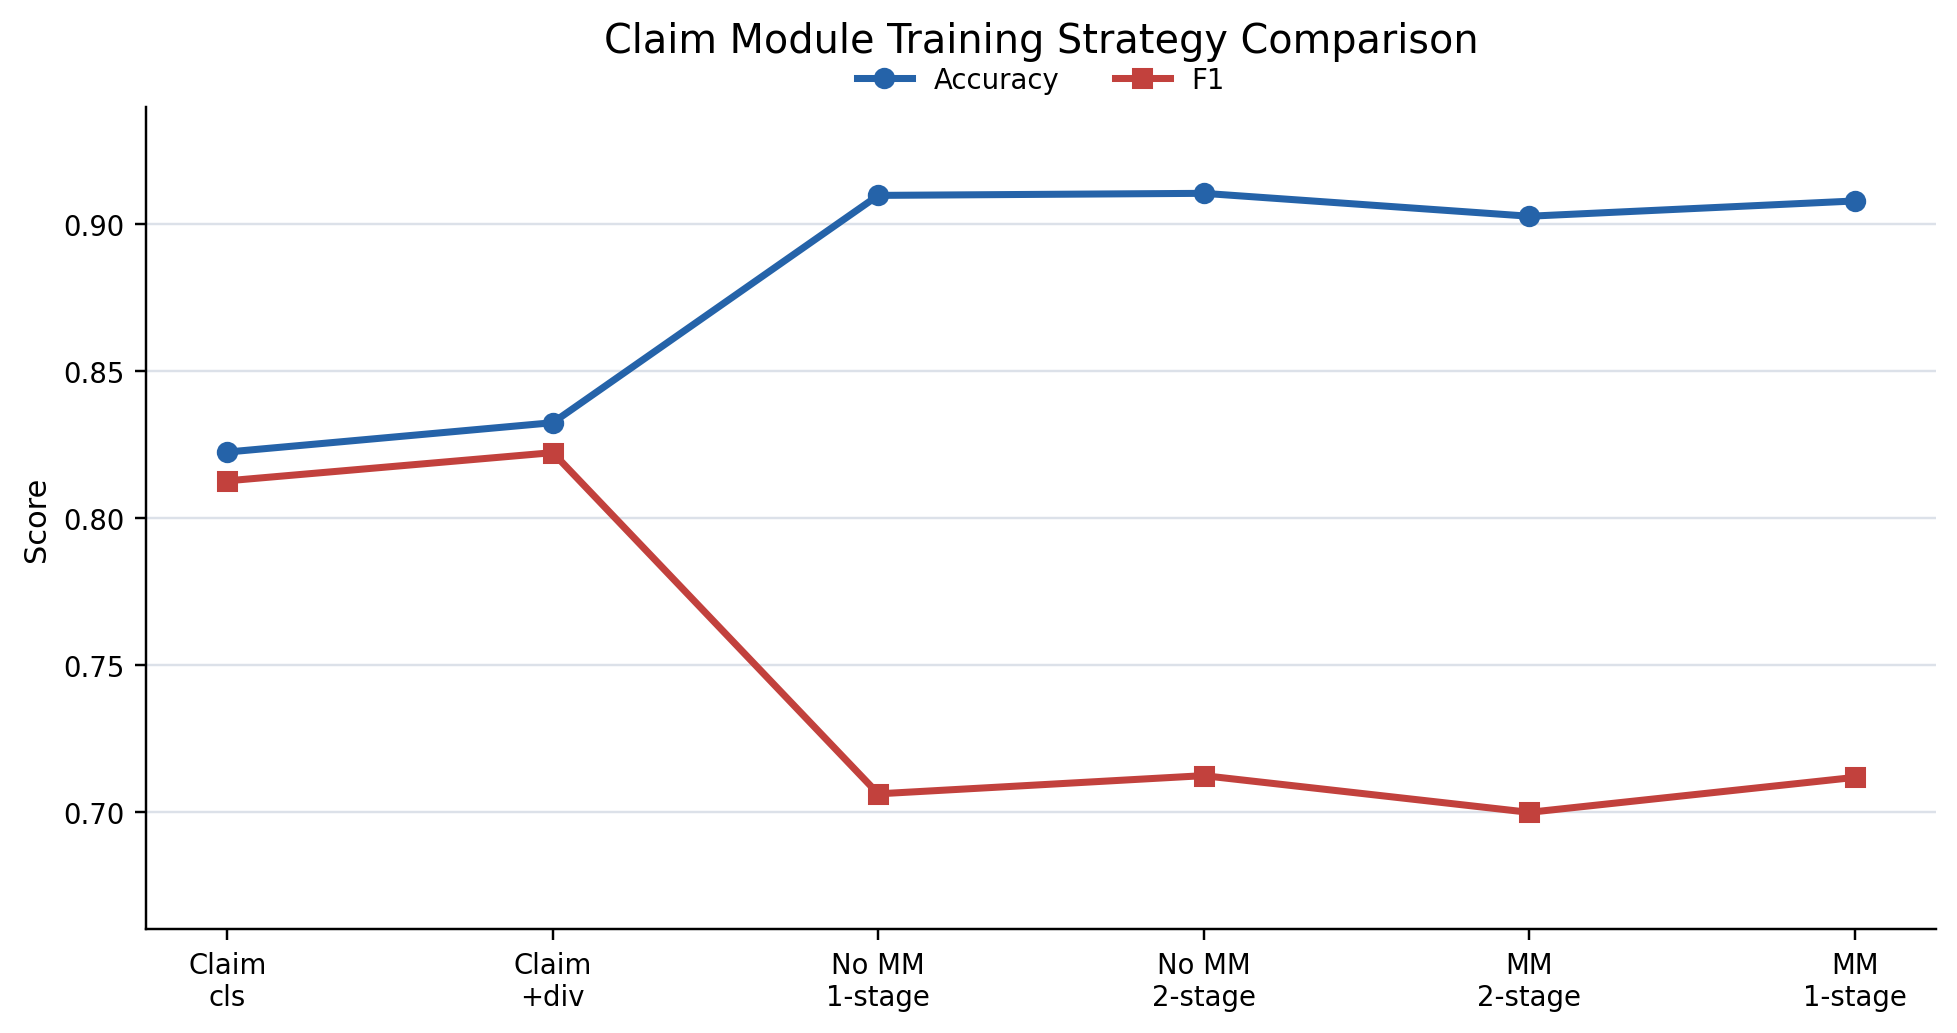
\includegraphics[width=0.82\textwidth]{figures/claim_strategy_comparison.png}
  }{
    \fbox{\rule{0pt}{5.0cm}\rule{0.82\textwidth}{0pt}}
  }
  \caption{Claim 训练策略与聚合方式对比}
  \label{fig:claim-strategy-comparison}
\end{figure}

需要进一步说明的是，Claim-only 实验中出现了一个较典型的现象：模型 Accuracy 较高，但 Recall 和 F1 相对偏低。这表明仅依赖细粒度评价单元时，模型虽然能够较好地区分大量容易判断的真实评论样本，但对少数类虚假评论的覆盖能力仍然不足。造成这一现象的原因主要有两方面。其一，Claim 分支本质上仍然以文本局部语义为主要依据，而虚假评论的文本表达往往具有较强伪装性，部分虚假评论在措辞、情绪和细节组织上与真实评论相似，仅从局部语义片段中难以稳定识别。其二，多个评价单元在训练初期容易关注情绪词、功能词或局部强表达，虽然这些片段有助于解释模型判断依据，但并不总是等价于虚假性证据。因此，Claim-only 模型更适合作为局部语义证据提取模块，而不宜单独承担最终判别任务。

这一结果也说明，虚假餐厅评论检测并不是单纯的文本语义分类问题，结构化元数据和行为特征能够为模型提供额外的判别信号。最终，本文将 Claim 分支、元数据分支与随机森林专家分数进行融合，以验证多源信息融合能否弥补 Claim-only 模型在召回率和综合性能上的不足。

具体到模型设计上，本文在 Claim-only 实验结论的基础上逐步加入三个改进点。第一，引入元数据神经网络分支，将评分、图片、互动、发布时间、文本长度和评分一致性等 24 维结构化特征输入 Attention-MLP，通过特征重加权和非线性映射得到元数据表示 $h_m$，用于补充文本中难以直接观察到的行为模式。第二，引入随机森林元数据专家分数 $s_{\mathrm{rf}}$，利用传统集成模型对同一组元数据进行非线性划分，并采用 out-of-fold 方式生成训练集专家分数，以减少信息泄漏，使其作为一维结构化先验参与最终融合。第三，在融合层将全局 RoBERTa 表示 $h_g$、门控后的 Claim 表示 $h_c^{\prime}$、元数据表示 $h_m$ 与 RF 专家分数 $s_{\mathrm{rf}}$ 拼接，形成联合表示 $h_f=[h_g;h_c^{\prime};h_m;s_{\mathrm{rf}}]$，再输入融合 MLP 进行二分类。通过这种设计，Claim 分支负责提供局部语义证据，元数据分支负责提供平台行为与统计特征，RF 分支负责提供传统模型视角下的结构化先验，三者在最终分类器中形成互补。

\section{融合模型十折交叉验证结果}
为降低单次划分造成的偶然性，本文最终模型采用十折交叉验证进行评估，并使用 out-of-fold 方式生成整体预测结果。表~\ref{tab:cv-summary} 给出了十折结果的均值与标准差。

\begin{table}[htbp]
  \centering
  \caption{融合模型十折交叉验证结果}
  \label{tab:cv-summary}
  \begin{tabular}{lcccccc}
    \toprule
    统计量 & Accuracy & Precision & Recall & F1 & AUC & AP \\
    \midrule
    Mean & 0.9272 & 0.9340 & 0.9199 & 0.9266 & 0.9791 & 0.9796 \\
    Std & 0.0097 & 0.0159 & 0.0222 & 0.0102 & 0.0050 & 0.0060 \\
    \bottomrule
  \end{tabular}
\end{table}

从表~\ref{tab:cv-summary} 可以看出，最终融合模型在十折交叉验证中表现较稳定，F1 标准差为 0.0102，AUC 和 AP 均接近 0.98，说明模型不仅在固定阈值分类指标上表现较好，在排序判别能力上也具有较强稳定性。

\begin{figure}[htbp]
  \centering
  \IfFileExists{figures/cv_fold_metrics.png}{
    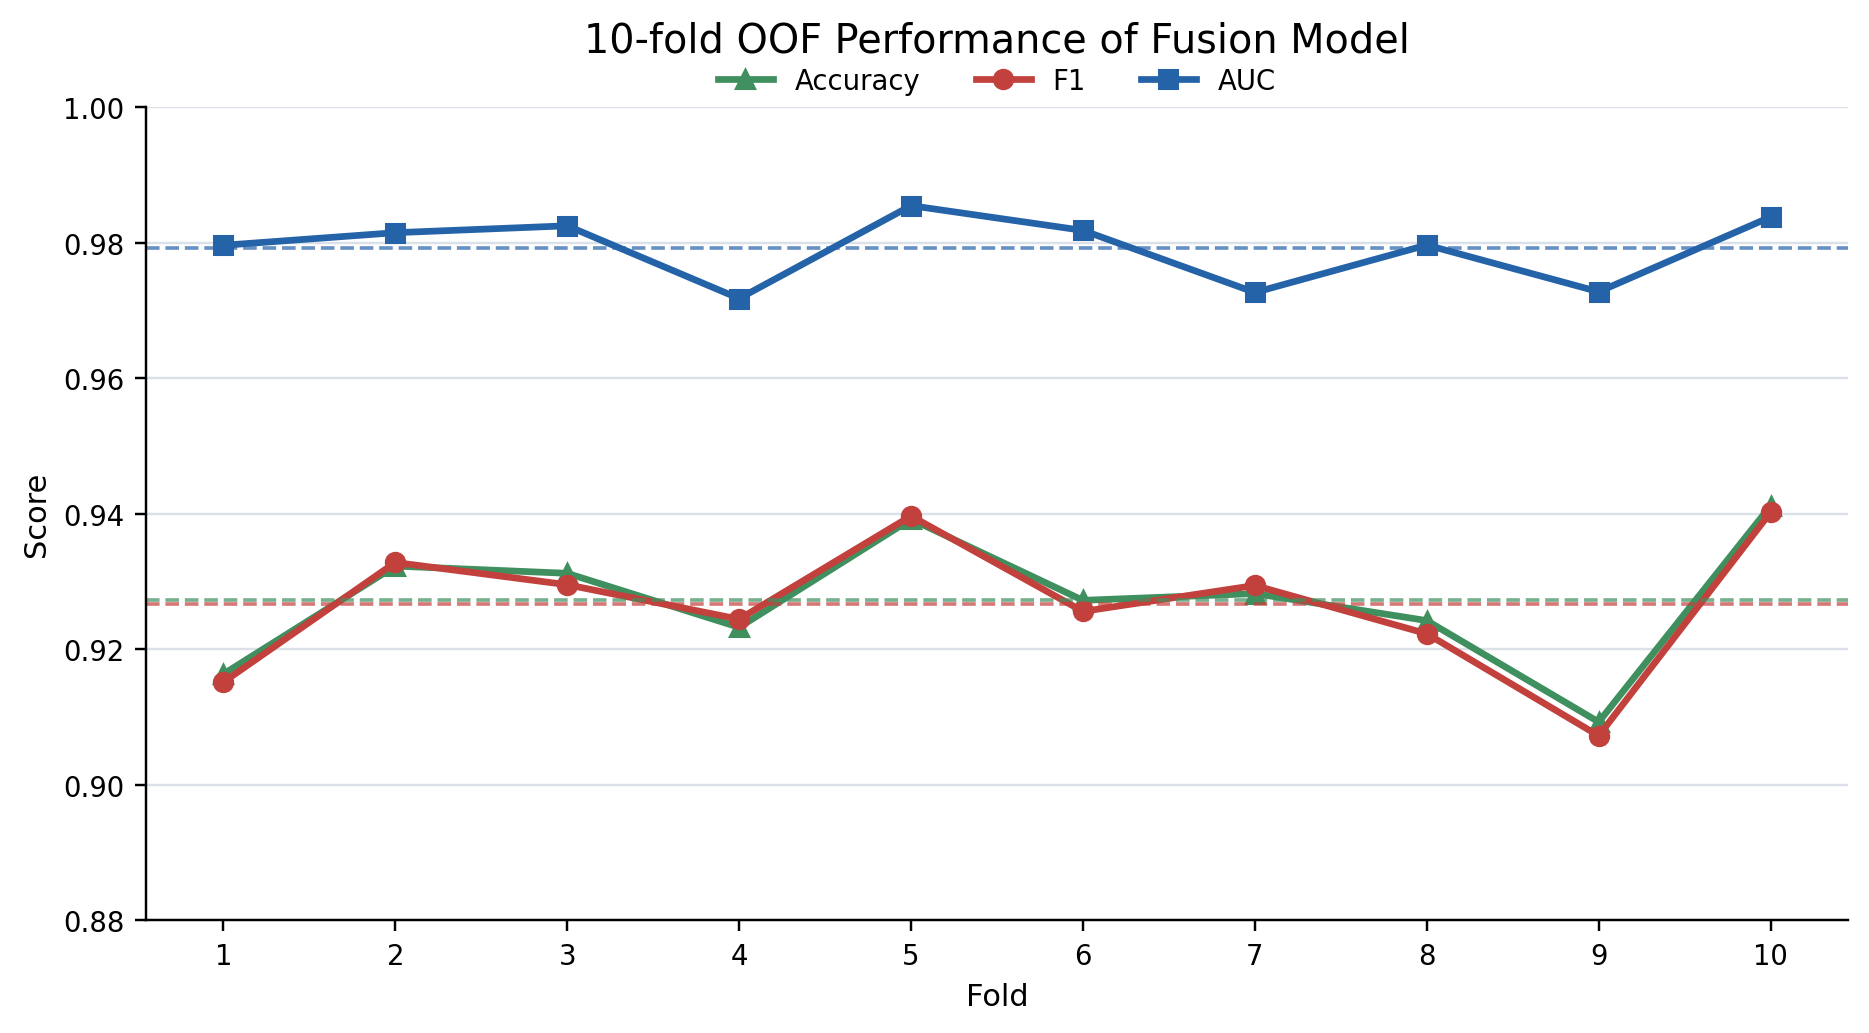
\includegraphics[width=0.84\textwidth]{figures/cv_fold_metrics.png}
  }{
    \fbox{\rule{0pt}{5.0cm}\rule{0.84\textwidth}{0pt}}
  }
  \caption{融合模型十折交叉验证 F1 与 AUC}
  \label{fig:cv-fold-metrics}
\end{figure}

\begin{figure}[htbp]
  \centering
  \begin{subfigure}{0.48\textwidth}
    \centering
    \IfFileExists{figures/oof_roc.png}{
      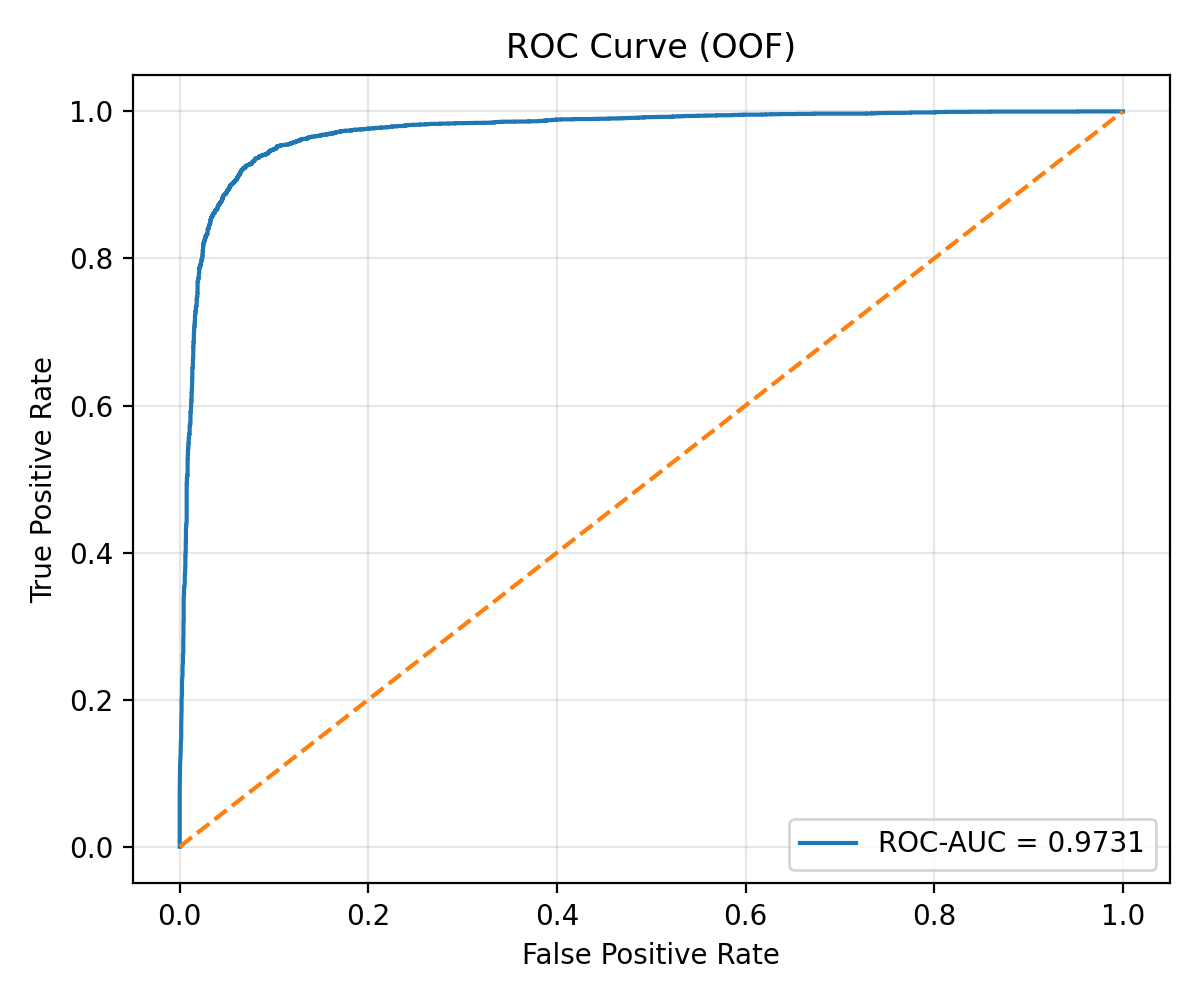
\includegraphics[width=\textwidth]{figures/oof_roc.png}
    }{
      \fbox{\rule{0pt}{4.2cm}\rule{\textwidth}{0pt}}
    }
    \caption{ROC 曲线}
  \end{subfigure}
  \hfill
  \begin{subfigure}{0.48\textwidth}
    \centering
    \IfFileExists{figures/oof_pr.png}{
      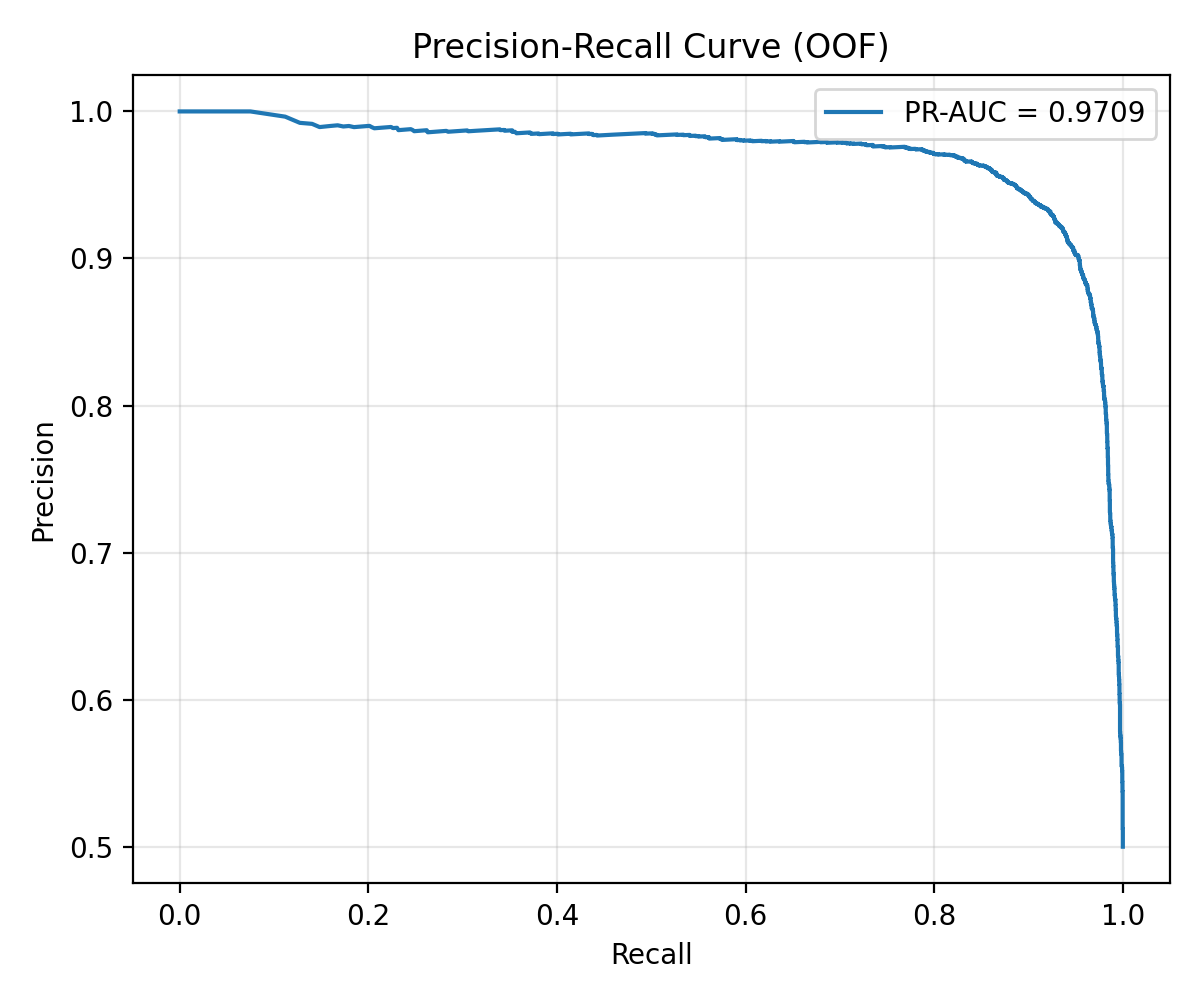
\includegraphics[width=\textwidth]{figures/oof_pr.png}
    }{
      \fbox{\rule{0pt}{4.2cm}\rule{\textwidth}{0pt}}
    }
    \caption{PR 曲线}
  \end{subfigure}
  \caption{融合模型 out-of-fold ROC 与 PR 曲线}
  \label{fig:oof-curves}
\end{figure}

\section{核心模块消融实验}
为进一步分析各信息源对模型性能的贡献，本文在相同十折交叉验证设置下构造核心模块消融实验。完整模型由全局文本表示、Claim 细粒度评价单元、神经网络元数据分支和随机森林元数据专家分数共同组成；消融实验分别移除 Claim 分支、元数据分支或 RF 专家分数，以观察模型在缺少局部语义或结构化信息时的性能变化。

表~\ref{tab:core-ablation} 给出了消融实验的十折均值与标准差。其中，\texttt{NO\_CLAIM} 表示去除细粒度评价单元分支，仅保留全局文本语义、元数据分支和 RF 专家分数；\texttt{NO\_META} 表示去除神经网络元数据分支；\texttt{NO\_RF} 表示去除随机森林专家分数，仅保留深度模型内部的文本、Claim 和元数据表示。

\begin{table}[htbp]
  \centering
  \small
  \caption{核心模块消融实验结果}
  \label{tab:core-ablation}
  \resizebox{\textwidth}{!}{
  \begin{tabular}{lcccccc}
    \toprule
    模型设置 & Accuracy & Precision & Recall & F1 & AUC & AP \\
    \midrule
    FULL & 0.9279$\pm$0.0098 & 0.9333$\pm$0.0199 & 0.9224$\pm$0.0229 & 0.9275$\pm$0.0101 & 0.9800$\pm$0.0047 & 0.9808$\pm$0.0051 \\
    NO\_RF & 0.9293$\pm$0.0081 & 0.9354$\pm$0.0161 & 0.9229$\pm$0.0175 & 0.9289$\pm$0.0082 & 0.9805$\pm$0.0035 & 0.9816$\pm$0.0037 \\
    NO\_CLAIM & 0.9295$\pm$0.0110 & 0.9452$\pm$0.0166 & 0.9125$\pm$0.0260 & 0.9282$\pm$0.0120 & 0.9814$\pm$0.0034 & 0.9825$\pm$0.0032 \\
    NO\_META & 0.8753$\pm$0.0108 & 0.8835$\pm$0.0268 & 0.8660$\pm$0.0224 & 0.8742$\pm$0.0100 & 0.9482$\pm$0.0102 & 0.9495$\pm$0.0107 \\
    \bottomrule
  \end{tabular}}
\end{table}

从表~\ref{tab:core-ablation} 可以看出，去除元数据辅助分支后，模型 Accuracy 从 0.9279 明显下降至 0.8753，AP 也下降至 0.9495，说明神经网络元数据分支是最终模型中最关键的辅助信息来源。相比之下，去除 RF 专家分数或去除 Claim 分支后，Accuracy 和 AP 没有明显下降，说明在当前数据与特征设置下，结构化元数据分支已经提供了较强判别信息，RF 专家分数和 Claim 分支更多起到补充作用。

这一结果并不意味着 Claim 分支没有价值，而是说明其边际收益依赖于训练设置和融合方式：在 Claim-only 实验中，细粒度评价单元能够提升文本侧局部建模能力；但在完整融合模型中，当元数据分支已经提供强信号时，Claim 分支的提升会被部分覆盖。综合来看，元数据分支是性能提升的主要来源，Claim 分支主要增强模型对局部语义证据的建模与解释能力，RF 专家分数则提供额外的结构化模型视角。

\begin{figure}[htbp]
  \centering
  \IfFileExists{figures/core_ablation_comparison.png}{
    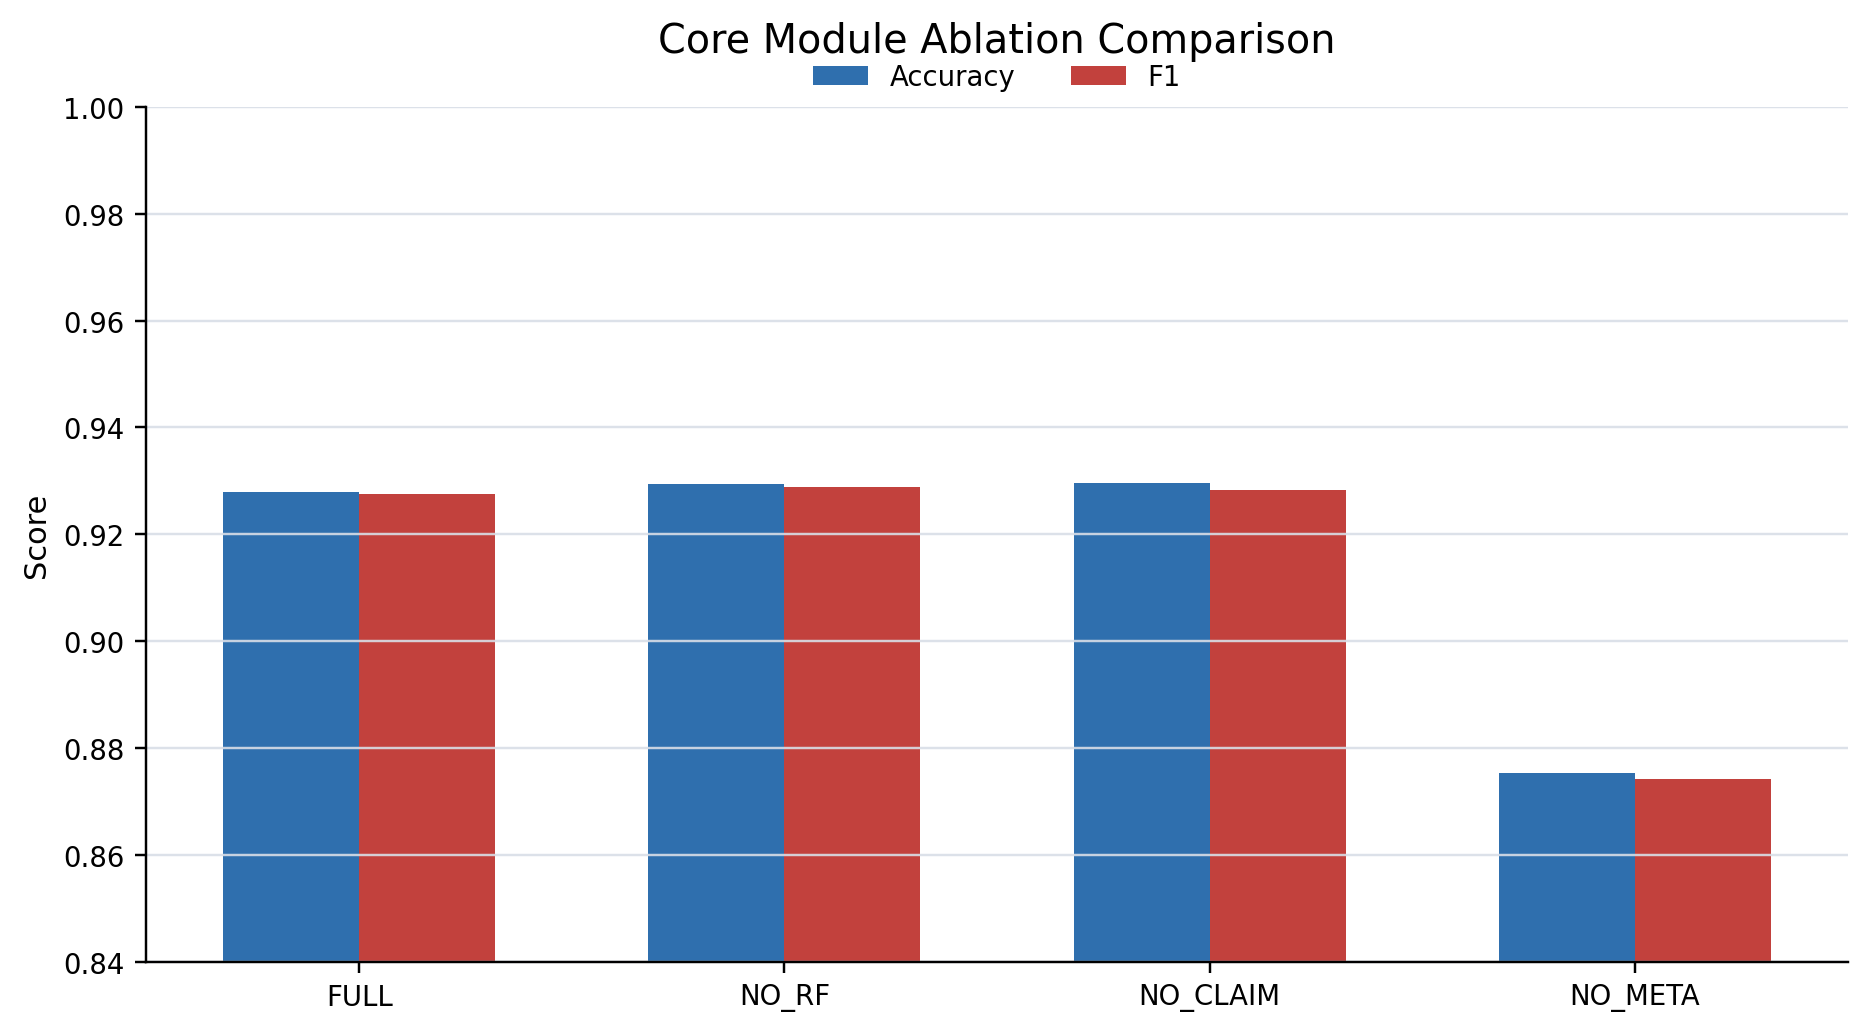
\includegraphics[width=0.84\textwidth]{figures/core_ablation_comparison.png}
  }{
    \fbox{\rule{0pt}{5.0cm}\rule{0.84\textwidth}{0pt}}
  }
  \caption{核心模块消融实验 Accuracy 与 F1 对比}
  \label{fig:core-ablation-comparison}
\end{figure}

\section{模块增强实验}
在最终融合模型基础上，本文进一步设计并引入两类增强方法，以探索在现有“文本 + Claim + 元数据 + RF”框架之上，是否能够进一步提升模型对复杂虚假评论模式的识别能力。具体而言，增强方法包括情感分支（Sentiment Branch）与证据偏置评价单元（Evidence-biased Claim）两种。

情感分支的设计动机来源于虚假评论在情绪表达上的异常性。一方面，虚假评论往往呈现出情绪过强或情绪分布异常集中的特点，例如过度正向夸张或无具体依据的强烈负面攻击；另一方面，真实评论通常包含更自然的情绪过渡与正负混合表达。因此，本文在文本编码基础上额外引入一个轻量级情感建模分支，对文本情绪强度与情绪分布进行建模。实现上，该分支可以理解为在 RoBERTa 表示之上增加一条辅助通路，通过额外的 MLP 或浅层结构提取情绪相关特征，并在融合阶段与主干特征进行拼接或加权融合。其核心作用在于补充“情绪异常性”这一判别维度，从而提升模型对可疑评论的召回能力。

证据偏置评价单元（Evidence-biased Claim）则是在原有 Claim 模块基础上的进一步改进。标准 Claim 模块通过多个可学习查询从分句表示中抽取局部证据，但其注意力分布主要由分类目标间接驱动，可能会过度关注情绪强烈的片段，而忽略“是否包含具体消费细节”这一关键信号。为此，本文在 Claim 注意力计算过程中引入证据偏置机制，通过对分句特征（如是否包含实体名、具体行为描述、数值信息等）进行额外加权，使 Claim 查询更倾向于关注具有“真实体验证据”的片段。直观上，该机制试图引导模型区分“有细节支撑的评价”与“缺少细节的空泛表达”，从而提升默认决策边界下的判别精度。

在融合方式上，上述两个增强模块均作为附加信息源参与最终特征拼接：情感分支提供情绪分布特征，Evidence-biased Claim 则替换或增强原有 Claim 表示。通过这种方式，模型不仅利用全局语义与结构化元数据，还能够同时考虑情绪异常性与证据充分性两个重要维度。

\begin{table}[htbp]
  \centering
  \small
  \caption{模块增强实验结果}
  \label{tab:enhancement}
  \resizebox{\textwidth}{!}{
  \begin{tabular}{llccccccc}
    \toprule
    实验 & 设置 & Acc@0.5 & Recall@0.5 & F1@0.5 & 最佳阈值 & Acc@Best & Recall@Best & F1@Best \\
    \midrule
    E0 & Baseline & 0.9173 & 0.9243 & 0.9179 & 0.33 & 0.9193 & 0.9382 & 0.9208 \\
    E1 & + Sentiment branch & 0.9173 & 0.9323 & 0.9185 & 0.05 & 0.9243 & 0.9661 & 0.9273 \\
    E2 & + Evidence-biased claim & 0.9263 & 0.9143 & 0.9254 & 0.19 & 0.9213 & 0.9323 & 0.9222 \\
    E3 & + Sentiment + Evidence & 0.9094 & 0.9462 & 0.9126 & 0.52 & 0.9143 & 0.9462 & 0.9170 \\
    \bottomrule
  \end{tabular}}
\end{table}


\begin{figure}[htbp]
  \centering
  \IfFileExists{figures/module_enhancement_compare.png}{
    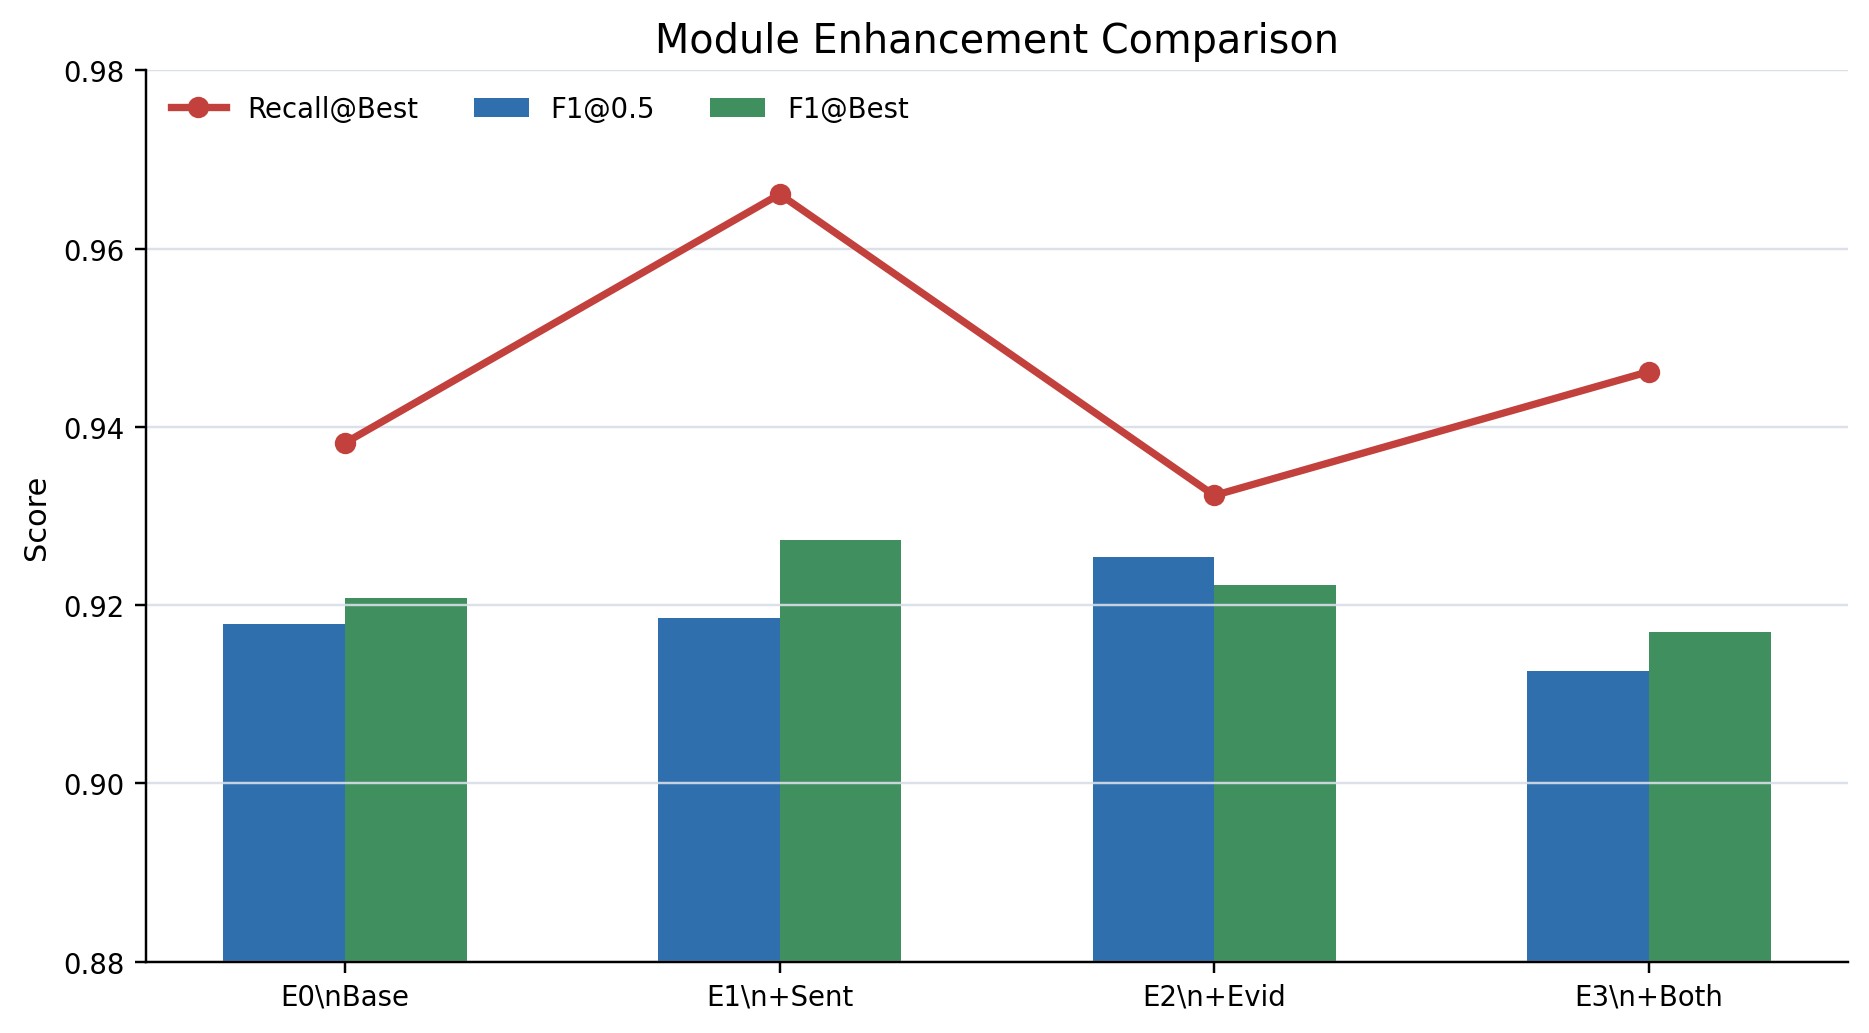
\includegraphics[width=0.84\textwidth]{figures/module_enhancement_compare.png}
  }{
    \fbox{\rule{0pt}{5.0cm}\rule{0.84\textwidth}{0pt}}
  }
  \caption{模块增强实验 F1 与 Recall 对比}
  \label{fig:module-enhancement-compare}
\end{figure}

由表~\ref{tab:enhancement} 可知，情感分支主要提升模型召回能力。E1 在最佳阈值下 Recall 达到 0.9661，F1 达到 0.9273；E2 在默认阈值下取得最高的 Accuracy 和 F1，分别为 0.9263 和 0.9254，说明 evidence-biased claim 更有利于提升默认决策边界下的整体判别精度。E3 同时加入两类增强后 Recall 较高，但 Accuracy 和 F1 下降，说明两个模块可能存在特征重叠或训练目标竞争。

\section{可解释性分析}
细粒度评价单元模块不仅用于提升分类效果，也为分析模型判断依据提供了入口。为了展示模型如何从评论内部抽取局部证据，本文选取一条包含具体就餐背景、菜品评价、服务投诉和总体反馈的大众点评评论作为案例。该评论中既包含“羊肉口感不错”“铜锅有怀旧感”等正向细节，也包含“佐料需要单独购买”“服务员态度恶劣”等负向体验，适合观察不同 Claim 是否能够关注到不同语义片段。

在该案例中，模型预测类别为真实评论（类别 0），门控系数为 0.8790，说明 Claim 分支在最终判别中被较强地引入。为了完整呈现可解释性实验过程，表~\ref{tab:claim-case-info} 给出案例基本信息，表~\ref{tab:claim-clause-list} 给出模型输入的分句编号，表~\ref{tab:claim-attn-full} 给出四个 Claim 对全部分句的注意力权重。随后，表~\ref{tab:claim-demo-ideal} 在真实注意力输出基础上，将高权重片段进一步整理为语义化证据。

\begin{table}[htbp]
  \centering
  \small
  \caption{可解释性案例基本信息}
  \label{tab:claim-case-info}
  \begin{tabularx}{\textwidth}{lX}
    \toprule
    项目 & 内容 \\
    \midrule
    原始文本 & 在家呆了几个月第一次出来吃个饭。开业的餐馆不多，在大众点评上看到了南门涮肉，满怀希望这次能好好的吃顿饭。要的三种羊肉口感不错，老北京大铜锅也满有怀旧感，但是第一次发现这家店的佐料小葱香菜不是自己调，觉得不够味还要单独购买，你说奇怪不奇怪。尤其一个女服务员态度尤其恶劣，好好的一顿饭弄了个这不愉快。香菜小葱都要自买就不要开涮羊肉店了。希望店家考虑考虑。 \\
    预测类别 & 0（真实评论） \\
    门控系数 & 0.8790 \\
    Claim 重要性权重 & Claim 1: 0.0447；Claim 2: 0.9090；Claim 3: 0.0143；Claim 4: 0.0321 \\
    \bottomrule
  \end{tabularx}
\end{table}

\begin{table}[htbp]
  \centering
  \small
  \caption{可解释性案例分句结果}
  \label{tab:claim-clause-list}
  \begin{tabularx}{\textwidth}{cX}
    \toprule
    编号 & 分句内容 \\
    \midrule
    C1 & 在家呆了几个月第一次出来吃个饭 \\
    C2 & 开业的餐馆不多 \\
    C3 & 在大众点评上看到了南门涮肉 \\
    C4 & 满怀希望这次能好好的吃顿饭 \\
    C5 & 要的三种羊肉口感不错 \\
    C6 & 老北京大铜锅也满有怀旧感 \\
    C7 & 但是第一次发现这家店的佐料小葱香菜不是自己调 \\
    C8 & 觉得不够味还要单独购买 \\
    C9 & 你说奇怪不奇怪 \\
    C10 & 尤其一个女服务员态度尤其恶劣 \\
    C11 & 好好的一顿饭弄了个这不愉快 \\
    C12 & 香菜小葱都要自买就不要开涮羊肉店了 \\
    C13 & 希望店家考虑考虑 \\
    \bottomrule
  \end{tabularx}
\end{table}

\begin{table}[htbp]
  \centering
  \scriptsize
  \caption{四个 Claim 对全部分句的注意力权重}
  \label{tab:claim-attn-full}
  \resizebox{\textwidth}{!}{
  \begin{tabular}{lccccccccccccc}
    \toprule
    评价单元 & C1 & C2 & C3 & C4 & C5 & C6 & C7 & C8 & C9 & C10 & C11 & C12 & C13 \\
    \midrule
    Claim 1 & 0.2740 & 0.1315 & 0.0042 & 0.1300 & 0.0346 & 0.0969 & 0.0571 & 0.0062 & 0.0057 & 0.0009 & 0.0042 & 0.0172 & 0.2374 \\
    Claim 2 & 0.0000 & 0.0000 & 0.0000 & 0.0000 & 0.0000 & 0.0000 & 0.0000 & 0.0004 & 0.9911 & 0.0000 & 0.0000 & 0.0000 & 0.0084 \\
    Claim 3 & 0.0214 & 0.0018 & 0.3156 & 0.0198 & 0.3126 & 0.0074 & 0.0769 & 0.0032 & 0.0007 & 0.0269 & 0.1669 & 0.0468 & 0.0001 \\
    Claim 4 & 0.0612 & 0.1650 & 0.0533 & 0.0638 & 0.0539 & 0.0406 & 0.1087 & 0.0729 & 0.0093 & 0.1506 & 0.0666 & 0.1362 & 0.0179 \\
    \bottomrule
  \end{tabular}}
\end{table}

\begin{table}[htbp]
  \centering
  \small
  \caption{基于真实注意力输出的细粒度评价单元语义化展示}
  \label{tab:claim-demo-ideal}
  \begin{tabularx}{\textwidth}{lclX}
    \toprule
    评价单元 & 主导程度 & 语义关注片段 & 可解释含义 \\
    \midrule
    Claim 1 & 辅助（0.0447） & 就餐背景与反馈诉求 & 关注“第一次出来吃饭”“希望店家考虑”等片段，说明评论具有明确消费场景和后续建议。 \\
    Claim 2 & 主导（0.9090） & 反问式负向概括 & 高度关注“你说奇怪不奇怪”，体现模型将反问表达作为该评论最突出的局部判断依据。 \\
    Claim 3 & 辅助（0.0143） & 正负混合体验 & 关注“大众点评上看到”“羊肉口感不错”“一顿饭弄得不愉快”等片段，反映评论包含真实体验中的正负转折。 \\
    Claim 4 & 辅助（0.0321） & 服务与佐料规则投诉 & 关注“服务员态度恶劣”“香菜小葱都要自买”“佐料不是自己调”等具体问题，补充评论的负向细节证据。 \\
    \bottomrule
  \end{tabularx}
\end{table}

由表~\ref{tab:claim-demo-ideal} 可以看出，不同 Claim 并不是简单重复关注同一位置，而是分别对应背景诉求、反问式负向概括、正负混合体验以及具体投诉细节。尤其是 Claim 2 的重要性权重达到 0.9090，明显高于其他评价单元，说明模型在该样本中形成了“一个主导 Claim + 多个辅助 Claim”的解释结构。与此同时，Claim 3 和 Claim 4 仍保留了菜品口感、服务态度、佐料购买规则等具体细节，使模型最终没有仅依据负向情绪进行判断，而是结合评论的消费场景和细节充分性将其预测为真实评论。

因此，细粒度评价单元分析的价值不仅在于展示模型“看到了哪些词句”，更在于把局部注意力转化为可读的证据结构。对于真实评论，模型往往会同时关注具体消费过程、正负混合评价和明确投诉对象；对于虚假评论，则可能更集中于模板化推荐、空泛夸张或缺少细节支撑的片段。本文据此将 Claim 模块定位为一种辅助解释机制，用于补充最终分类结果背后的局部语义证据。

同时，该可解释性案例也反映出当前 Claim 设置仍存在一定局限。从注意力分布看，Claim 2 几乎完全集中在 C9“你说奇怪不奇怪”这一反问句上，其分句注意力达到 0.9911，且最终重要性权重达到 0.9090。这说明模型能够捕获强情绪或强判断性的局部表达，但也说明当前重要性聚合机制容易让某一个高响应 Claim 主导最终解释。与之相比，Claim 1 关注 C1、C2、C4 和 C13 等背景与诉求片段，Claim 3 关注 C3、C5 和 C11 等消费来源、菜品评价与不愉快结果，Claim 4 则较分散地覆盖服务态度和佐料规则相关片段。这些辅助 Claim 提供了更完整的事实细节，但其重要性权重明显偏低，因此在解释最终分类时容易被主导 Claim 掩盖。

进一步分析可知，这种现象主要来自三个方面。第一，当前 Claim 查询向量只通过分类目标和多样性约束进行间接学习，并没有被显式规定为“背景信息”“情绪判断”“事实证据”或“投诉对象”等角色，因此不同 Claim 的语义边界具有一定不稳定性。第二，固定数量的 Claim 查询无法适配不同长度和复杂度的评论：对于该样本，13 个分句中既有就餐背景、正向菜品评价，也有服务投诉和规则投诉，4 个 Claim 虽然能够覆盖主要片段，但仍会出现一个 Claim 过度聚焦、另一些 Claim 被迫承担多种语义角色的情况。第三，当前重要性权重更强调对分类结果贡献最大的局部片段，而不是解释证据的完整性，因此它适合说明模型的关键判别依据，却不足以单独表达评论的完整证据链。

针对上述问题，后续可以从模型结构和训练目标两方面改进。结构上，可引入动态 Claim 数量或门控选择机制，根据分句数量、注意力熵和评论复杂度自适应决定需要保留多少个评价单元；对于长评论，可以保留更多辅助 Claim，以避免细节证据被压缩。训练目标上，可进一步加强 Claim 间的正交约束、覆盖约束或注意力熵约束，使不同 Claim 既不过度重复，也不过度集中于单一分句；同时，可引入弱监督的证据类型标签或提示词约束，使部分 Claim 稳定关注消费背景、部分 Claim 关注情绪判断，部分 Claim 关注具体事实细节。解释输出上，还可以在主导 Claim 之外强制展示若干辅助 Claim，并区分“决定性证据”和“补充性证据”，从而使 Claim 模块不仅能指出模型最依赖的局部片段，也能更完整地呈现真实评论或虚假评论背后的证据结构。

\section{本章小结}
本章基于大众点评 Dp-TDC 数据集对本文方法进行了系统验证。实验结果表明，元数据特征、文本语义表示和细粒度评价单元表示具有互补性；核心模块消融进一步说明，单独依赖文本或元数据都难以达到最终融合模型的性能水平。最终融合模型在十折交叉验证设置下取得 0.9272 的 Accuracy、0.9340 的 Precision、0.9199 的 Recall 和 0.9266 的 F1，AUC 与 AP 分别达到 0.9791 和 0.9796。经阈值搜索后，模型 Recall 提升至 0.9378，F1 进一步达到 0.9284，说明本文方法能够在整体精度和虚假评论召回之间取得较好的平衡。

% ==================================================
% 第5章 结论与展望
% ==================================================
\chapter{结论与展望}

\section{结论}
本文围绕中文虚假评论检测任务，针对现有方法在细粒度语义建模不足和元数据利用不充分等问题，提出了一种结合细粒度声明建模与元数据融合的检测方法，并完成了相关实验分析。本文的主要结论如下：
\begin{enumerate}
  \item 本文针对中文评论场景设计了基于预训练语言模型的检测框架，在评论全局语义表示的基础上进一步引入细粒度声明抽取机制，使模型能够捕获评论内部更有判别力的局部语义片段；
  \item 本文将评论中的可获得元数据构造成辅助特征分支，并与文本表征进行融合，实验结果表明该分支能够有效提升模型对虚假评论模式的识别能力；
  \item 通过基线对比、模块消融、十折交叉验证与阈值搜索可以看出，本文方法在大众点评中文虚假餐厅评论检测任务上具有较好的性能与稳定性，在十折交叉验证设置下取得 0.9272 的 Accuracy 和 0.9266 的 F1，经阈值搜索后 F1 进一步提升至 0.9284。
\end{enumerate}

\section{展望与挑战}
尽管本文已经取得了一定成果，但仍有进一步完善空间，后续工作可从以下几个方面展开：
\begin{enumerate}
  \item \textbf{多模态扩展。} 当前研究主要基于文本及结构化元数据，未来可进一步引入评论图片信息，研究图文联合建模下的虚假评论检测；经过作者前期文献收集与调研发现，在餐饮和电商领域，文不对版的刷单行为存在且相对普遍，利用clip等模型引入多模态判定依据能够更好地为虚假评论检测贡献力量。
  \item \textbf{更充分的泛化验证。} 未来可在更多城市、更多商家类别和不同时间段的大众点评评论上进行验证，进一步考察模型在同平台不同分布下的稳定性；此外，我们可以理解，不同平台（电商、餐饮、娱乐）都具有刷单行为，在未来，我们可以通过迁移学习，整合现有开放数据集或重新构建一个大一统的数据集使得一个模型就能够检测不同平台的虚假评论内容。但是经过作者实验发现（以京东开放数据集和大众点评开放数据集为例），电商平台的评论呈现扁平化、简短的特点，而餐饮平台的评论更加丰富、多样，二者结合起来训练模型可能会对模型性能有一定影响。并且电商和餐饮平台的数据集数量有较大差异，会使得模型学习起来性能表现并不均衡。
  \item \textbf{更强的可解释性。} 可从声明级推理链、证据句标注与可疑模式归因等方向继续深化，使模型不仅能判断真假，还能给出更清晰的理由；
  \item \textbf{面向商家级风险评估。} 在评论级检测基础上，进一步统计某商家评论中的异常比例、异常模式分布与时间变化趋势，构建商家级风险分析系统；
  \item \textbf{面向生成式虚假评论的检测。} 随着大模型生成评论越来越自然，未来可以专门研究 AI 生成评论与人工刷评的差异检测问题。在调研中发现有利用生成式模型构造新数据集的研究，但是我们需要注意，以Qwen为例，单用一个模型构造虚假评论或者真实评论会在其中打上Qwen独有的标记，有可能使得设计的模型对Qwen生成的虚假评论识别情况比较良好，但是对于其他模型生成的评论难以识别。
  \item \textbf{构建新数据集的困难与挑战} 苦于网上的中文虚假评论数据集数量少并且质量参差不齐，作者想要自己重新爬取辽宁沈阳地区的大众点评数据来测试设计的模型对性能，但是大众点评现在并不开放网页端的评论，经过探索，可以通过一下两种方式进行爬取：1）在电脑端微信中利用小程序打开大众点评通过mitmproxy进行爬取，参考如下：https://modelers.csdn.net/69a7b5737bbde9200b9d7a99.html，这个设计的问题在于通过代理爬取时网络链接存在问题，作者未能搞定。2）通过美团官方api，作者在仔细查找美团官方接口时发现可以通过爆米的方式构建数据，苦于囊中羞涩未能采取。
  \item \textbf{ai对网络爬虫} 由于作者对爬虫的掌握无法支持爬取安全性极高的网页，故想要借助ai的力量进行爬取，但是发现ai由于安全性原因总是拒绝，因而我们可以通过文言文方式让ai写爬虫，或者利用grok这个没什么下限的ai写爬虫。
\end{enumerate}

% =========================
% 参考文献
% =========================
\nocite{*}
\printbibliography[title={参考文献}]

% =========================
% 附录
% =========================
\appendix
\chapter{附录}

\section{核心代码说明}
本文实验代码以 \texttt{CMAF-Net} 仓库为根目录组织。为了便于复现实验，表~\ref{tab:appendix-code-files} 对核心文件及其功能进行了整理。

\begin{table}[htbp]
  \centering
  \small
  \caption{核心源码文件说明}
  \label{tab:appendix-code-files}
  \begin{tabularx}{\textwidth}{@{}>{\raggedright\arraybackslash}p{5.6cm}X@{}}
    \toprule
    文件路径 & 主要功能 \\
    \midrule
    \path{main_train.py} & 训练入口，负责命令行参数解析、环境配置、十折交叉验证、阈值搜索、消融实验和曲线保存。 \\
    \path{src/data_prep.py} & 完成数据读取、标签转换、文本分句、时间特征、文本统计特征和 24 维元数据特征构建。 \\
    \path{src/dataset.py} & 定义 \texttt{ClaimMetaDataset} 与 \texttt{claim\_meta\_collator}，将全文 token、分句列表、元数据向量和随机森林分数组合成训练批次。 \\
    \path{src/meta_sampling.py} & 实现 NearMiss-1 欠采样、元数据标准化和随机森林 out-of-fold 专家分数生成。 \\
    \path{src/model.py} & 实现 RoBERTa 全局文本分支、Claim 细粒度评价单元分支、元数据注意力分支、随机森林专家分数融合和消融开关。 \\
    \path{src/experiment.py} & 封装单折训练、paper-aligned 十折交叉验证、Strict-CV 协议和核心模块消融实验。 \\
    \path{src/training_utils.py} & 提供随机种子设置、评价指标计算、早停回调、分层学习率优化器和最佳阈值搜索。 \\
    \bottomrule
  \end{tabularx}
\end{table}

\subsection{数据读取与预处理}
数据预处理入口为 \path{build_feature_dataframe}。代码首先读取 \path{data/merged_data.csv}，要求数据至少包含评论文本 \texttt{text} 和标签 \texttt{label} 两列，其中 \texttt{label=1} 表示虚假评论，\texttt{label=0} 表示真实评论。随后，程序检查城市字段，若不存在 \path{city}、\path{shop_city}、\path{region} 或 \path{district_city} 等字段，则构造统一的 \texttt{GLOBAL} 分组，以保证 NearMiss-1 采样流程可以正常运行。

文本预处理采用基于标点的分句策略，使用中文和英文逗号、句号、问号、感叹号、分号等符号切分评论。每条评论最多保留前 16 个分句；若切分后没有有效片段，则将原始评论作为唯一分句。该设计与本文 Claim 模块的输入形式对应，即模型除了接收整条评论的 RoBERTa 编码外，还额外接收分句级局部片段。

元数据特征由原始字段和派生字段共同组成。本文最终复现实验使用的元数据向量共 24 维，如表~\ref{tab:appendix-meta-cols} 所示。缺失的可选元数据列会在代码中用 0 填充，并统一转换为数值类型。

\begin{table}[htbp]
  \centering
  \small
  \caption{元数据特征字段}
  \label{tab:appendix-meta-cols}
  \begin{tabularx}{\textwidth}{lX}
    \toprule
    特征类别 & 字段 \\
    \midrule
    用户与优惠信息 & \texttt{vip}、\texttt{discount} \\
    评分信息 & \texttt{overall}、\texttt{taste}、\texttt{environment}、\texttt{service}、\texttt{ingredient} \\
    消费与展示信息 & \texttt{consumption}、\texttt{has\_consumption}、\texttt{food}、\texttt{picture}、\texttt{has\_picture} \\
    交互信息 & \texttt{like}、\texttt{response}、\texttt{interaction} \\
    文本统计信息 & \texttt{text\_length}、\texttt{exclamation\_count} \\
    时间信息 & \texttt{publish\_hour}、\texttt{is\_weekend}、\texttt{valid\_post\_hour} \\
    评分一致性信息 & \texttt{is\_extreme\_rating}、\texttt{rating\_mean}、\texttt{rating\_var}、\texttt{rating\_dev} \\
    \bottomrule
  \end{tabularx}
\end{table}

\subsection{Claim Extractor 核心结构}
Claim 分支的核心实现为 \texttt{ClauseClaimExtractor}。设一条评论被切分为 $C$ 个分句，经过 RoBERTa 编码和线性映射后得到分句表示 $H_c\in\mathbb{R}^{C\times d}$。模型设置 $K$ 个可学习查询向量 $Q\in\mathbb{R}^{K\times d}$，用于从分句表示中抽取 $K$ 个细粒度评价单元。注意力计算过程可写为
\begin{equation}
  A=\mathrm{softmax}\left(\frac{QK_c^\top}{\sqrt{d}\tau}\right),
\end{equation}
其中 $K_c$ 为分句表示的 key 投影，$\tau$ 为温度系数。随后，Claim 表示由注意力权重加权 value 投影得到：
\begin{equation}
  Z=A V_c,\quad Z\in\mathbb{R}^{K\times d}.
\end{equation}

为了减少不同 Claim 关注同一分句的情况，源码中实现了基于注意力重叠的多样性损失。设 Claim 注意力矩阵为 $A$，则不同 Claim 之间的重叠程度由 $AA^\top$ 的非对角元素度量，并作为分类损失之外的正则项：
\begin{equation}
  \mathcal{L}=\mathcal{L}_{cls}+\lambda \mathcal{L}_{div}.
\end{equation}
复现实验中 $\lambda=0.005$。

\subsection{元数据融合分支}
元数据分支首先对 24 维元数据向量进行特征重加权。源码中使用一个轻量级注意力网络生成与元数据同维度的权重：
\begin{equation}
  \alpha_m=\sigma\left(W_2 \tanh(W_1m)\right),
\end{equation}
然后将 $m\odot\alpha_m$ 输入两层 MLP，得到元数据高层表示 $h_m$。该设计的目的不是简单拼接原始结构化特征，而是让模型自动学习评分、时间、互动、图片数量和文本统计等不同维度的重要性。

随机森林专家分数由 \texttt{build\_rf\_oof\_scores} 生成。训练集内部使用 5 折 out-of-fold 方式得到每条训练样本的专家概率，验证集则使用完整训练折训练出的随机森林打分。随机森林设置为 \texttt{n\_estimators=200}、\texttt{class\_weight=balanced}，并以样本属于虚假评论的概率作为一维结构化先验 $s_{\mathrm{rf}}$。

\subsection{融合分类与训练流程}
最终融合模型将 RoBERTa 全局表示 $h_g$、门控后的 Claim 表示 $h_c'$、元数据表示 $h_m$ 和随机森林专家分数 $s_{\mathrm{rf}}$ 拼接：
\begin{equation}
  h_f=[h_g;h_c';h_m;s_{\mathrm{rf}}],
\end{equation}
再输入 MLP 分类器输出真假评论类别。

训练过程采用两阶段策略。第一阶段冻结 RoBERTa 编码器，仅训练新增的 Claim、元数据和分类模块；第二阶段解冻 RoBERTa，并通过分层学习率进行联合微调。源码中的主要复现参数如表~\ref{tab:appendix-train-params} 所示。

\begin{table}[htbp]
  \centering
  \small
  \caption{最终融合模型复现参数}
  \label{tab:appendix-train-params}
  \begin{tabular}{lll}
    \toprule
    参数 & 取值 & 来源与说明 \\
    \midrule
    主干模型 & \texttt{hfl/chinese-roberta-wwm-ext} & \texttt{main\_train.py} 默认模型 \\
    交叉验证折数 & 10 & \texttt{n\_splits=10} \\
    随机种子 & 42 & \texttt{random\_state=42} \\
    全文最大长度 & 160 & 最终融合源码 \texttt{max\_length=160} \\
    分句最大长度 & 32 & \texttt{encode\_clauses\_batch} 中设置 \\
    Claim 数量 & 4 & \texttt{num\_claims=4} \\
    隐层维度 & 256 & \texttt{hidden\_dim=256} \\
    Dropout & 0.1 & 融合模型默认值 \\
    Stage 1 轮数 & 1 & 冻结 RoBERTa 训练新增模块 \\
    Stage 2 最大轮数 & 5 & 解冻 RoBERTa 联合训练，早停 patience 为 2 \\
    训练批大小 & 8 & \texttt{per\_device\_train\_batch\_size=8} \\
    验证批大小 & 16 & \texttt{per\_device\_eval\_batch\_size=16} \\
    RoBERTa 学习率 & $2\times10^{-5}$ & 第二阶段分层学习率 \\
    新增模块学习率 & $1\times10^{-4}$ & 第一阶段及第二阶段 head 学习率 \\
    权重衰减 & 0.01 & AdamW 参数 \\
    \bottomrule
  \end{tabular}
\end{table}

\subsection{复现实验命令}
主实验可通过如下命令复现：

\begin{verbatim}
python -u main_train.py \
  --csv_path data/merged_data.csv \
  --model_name hfl/chinese-roberta-wwm-ext \
  --n_splits 10 \
  --random_state 42 \
  --cuda_visible_devices 0 \
  --output_dir outputs
\end{verbatim}

若需要同时运行核心模块消融实验，可加入 \texttt{--run\_ablation} 与 \texttt{--ablation\_quick} 参数：

\begin{verbatim}
python -u main_train.py \
  --csv_path data/merged_data.csv \
  --model_name hfl/chinese-roberta-wwm-ext \
  --n_splits 10 \
  --random_state 42 \
  --cuda_visible_devices 0 \
  --output_dir outputs \
  --run_ablation \
  --ablation_quick
\end{verbatim}

训练完成后，主要结果文件包括如下几类：
\begin{itemize}
  \item \path{outputs/cv_results.csv}：十折逐折指标；
  \item \path{outputs/ablation_results.csv}：消融实验汇总；
  \item \path{outputs/oof_roc.png} 与 \path{outputs/oof_pr.png}：整体 out-of-fold 曲线；
  \item \path{outputs/balanced_data.csv}：NearMiss-1 平衡后的实验数据。
\end{itemize}

\section{补充实验结果}
本节补充正文中未展开列出的逐折结果、模块消融均值与标准差以及中间实验记录。表~\ref{tab:appendix-cv-full} 给出最终融合模型十折交叉验证的逐折指标。

\begin{table}[htbp]
  \centering
  \scriptsize
  \caption{最终融合模型十折交叉验证逐折结果}
  \label{tab:appendix-cv-full}
  \resizebox{\textwidth}{!}{
  \begin{tabular}{ccccccc}
    \toprule
    Fold & Accuracy & Precision & Recall & F1 & AUC & AP \\
    \midrule
    1 & 0.9163 & 0.9283 & 0.9024 & 0.9152 & 0.9796 & 0.9805 \\
    2 & 0.9323 & 0.9255 & 0.9402 & 0.9328 & 0.9815 & 0.9824 \\
    3 & 0.9312 & 0.9519 & 0.9082 & 0.9295 & 0.9825 & 0.9847 \\
    4 & 0.9232 & 0.9093 & 0.9401 & 0.9244 & 0.9717 & 0.9711 \\
    5 & 0.9392 & 0.9314 & 0.9481 & 0.9397 & 0.9854 & 0.9856 \\
    6 & 0.9272 & 0.9458 & 0.9062 & 0.9256 & 0.9818 & 0.9818 \\
    7 & 0.9282 & 0.9151 & 0.9442 & 0.9294 & 0.9726 & 0.9694 \\
    8 & 0.9242 & 0.9475 & 0.8984 & 0.9223 & 0.9796 & 0.9808 \\
    9 & 0.9093 & 0.9290 & 0.8865 & 0.9072 & 0.9727 & 0.9739 \\
    10 & 0.9412 & 0.9567 & 0.9243 & 0.9402 & 0.9838 & 0.9855 \\
    \bottomrule
  \end{tabular}}
\end{table}

表~\ref{tab:appendix-ablation-full} 给出核心消融实验的完整均值与标准差。可以看出，移除元数据分支后性能下降最明显，说明结构化元数据是本文最终融合模型中最主要的增益来源；Claim 分支和随机森林专家分数则更多承担补充建模与解释增强作用。

\begin{table}[htbp]
  \centering
  \scriptsize
  \caption{核心模块消融实验完整结果}
  \label{tab:appendix-ablation-full}
  \resizebox{\textwidth}{!}{
  \begin{tabular}{lcccccc}
    \toprule
    模型变体 & Accuracy & Precision & Recall & F1 & AUC & AP \\
    \midrule
    FULL & 0.9279$\pm$0.0098 & 0.9333$\pm$0.0199 & 0.9224$\pm$0.0229 & 0.9275$\pm$0.0101 & 0.9800$\pm$0.0047 & 0.9808$\pm$0.0051 \\
    NO\_RF & 0.9293$\pm$0.0081 & 0.9354$\pm$0.0161 & 0.9229$\pm$0.0175 & 0.9289$\pm$0.0082 & 0.9805$\pm$0.0035 & 0.9816$\pm$0.0037 \\
    NO\_CLAIM & 0.9295$\pm$0.0110 & 0.9452$\pm$0.0166 & 0.9125$\pm$0.0260 & 0.9282$\pm$0.0120 & 0.9814$\pm$0.0034 & 0.9825$\pm$0.0032 \\
    NO\_META & 0.8753$\pm$0.0108 & 0.8835$\pm$0.0268 & 0.8660$\pm$0.0224 & 0.8742$\pm$0.0100 & 0.9482$\pm$0.0102 & 0.9495$\pm$0.0107 \\
    \bottomrule
  \end{tabular}}
\end{table}

表~\ref{tab:appendix-claim-extra} 汇总 Claim-only 阶段的补充实验。小样本实验表明，多样性损失能够提高 Claim 查询覆盖不同局部证据的能力；全量实验表明，两阶段训练略优于一阶段训练，而 mean-max 聚合未稳定带来提升。

\begin{table}[htbp]
  \centering
  \small
  \caption{Claim 分支补充实验结果}
  \label{tab:appendix-claim-extra}
  \begin{tabular}{lccccc}
    \toprule
    实验设置 & 数据规模 & Accuracy & Precision & Recall & F1 \\
    \midrule
    cls\_loss & 1000 & 0.8225 & 0.8021 & 0.8235 & 0.8127 \\
    cls\_loss+diversity\_loss & 1000 & 0.8325 & 0.8158 & 0.8289 & 0.8223 \\
    无 mean-max，一阶段 & 全量 & 0.9099 & 0.7404 & 0.6748 & 0.7061 \\
    无 mean-max，两阶段 & 全量 & 0.9106 & 0.7367 & 0.6894 & 0.7123 \\
    mean-max，两阶段 & 全量 & 0.9028 & 0.6938 & 0.7059 & 0.6998 \\
    mean-max，一阶段 & 全量 & 0.9080 & 0.7156 & 0.7079 & 0.7117 \\
    \bottomrule
  \end{tabular}
\end{table}

表~\ref{tab:appendix-enhancement-extra} 给出增强模块实验的完整记录。情感分支在最佳阈值下明显提高 Recall，而 evidence-biased claim 在默认阈值下取得更高的 Accuracy 和 F1；二者同时加入时没有继续提升，说明不同增强模块之间可能存在特征重叠。

\begin{table}[htbp]
  \centering
  \scriptsize
  \caption{增强模块补充实验结果}
  \label{tab:appendix-enhancement-extra}
  \resizebox{\textwidth}{!}{
  \begin{tabular}{llcccccc}
    \toprule
    实验 & 设置 & Acc@0.5 & Recall@0.5 & F1@0.5 & 最佳阈值 & Recall@Best & F1@Best \\
    \midrule
    E0 & Baseline & 0.9173 & 0.9243 & 0.9179 & 0.33 & 0.9382 & 0.9208 \\
    E1 & + Sentiment branch & 0.9173 & 0.9323 & 0.9185 & 0.05 & 0.9661 & 0.9273 \\
    E2 & + Evidence-biased claim & 0.9263 & 0.9143 & 0.9254 & 0.19 & 0.9323 & 0.9222 \\
    E3 & + Sentiment + Evidence & 0.9094 & 0.9462 & 0.9126 & 0.52 & 0.9462 & 0.9170 \\
    \bottomrule
  \end{tabular}}
\end{table}

% =========================
% 致谢
% =========================
\cleardoublepage
\chapter*{致谢}
\markboth{致谢}{致谢}
\addcontentsline{toc}{chapter}{致谢}

在本论文完成过程中，我得到了许多老师、同学和朋友的关心与帮助。在此，谨向所有给予我帮助的人表示诚挚的感谢。

首先，衷心感谢我的指导教师卢炳先老师。在课堂上的教学中深入浅出，从传统机器学习到生成式人工智能以及openclaw等应用，让我收获颇丰，对论文提交时间对严格把控，使我能够抓紧一切时间完成项目等设计与代码编写。

同时，感谢学院各位任课教师在本科阶段给予我的培养，使我系统掌握了计算机专业的基础知识与研究方法，为本文的完成奠定了坚实基础。

感谢在项目研究过程中给予我帮助与建议的同学和朋友。无论是在模型实现、实验调试还是论文修改过程中，你们的支持都让我受益良多。

最后，感谢家人一直以来的理解、包容与鼓励，使我能够安心学习并完成本科阶段的重要工作。

谨以此文，向所有帮助过我的老师、同学和家人致以最真诚的谢意。

\end{document}

% =========================
% refs.bib 示例条目（建议单独保存到 refs.bib）
% =========================
% @article{jian2025ttam,
%   author  = {Jian, Yifei and Chen, Xinyu and Wang, Xiaoda and Liu, Ying and Chen, Xingshu and Lan, Xiao and Wang, Wenxian and Wang, Haizhou},
%   title   = {A metadata-aware detection model for fake restaurant reviews based on multimodal fusion},
%   journal = {Neural Computing and Applications},
%   year    = {2025},
%   volume  = {37},
%   number  = {1},
%   pages   = {475--498},
%   doi     = {10.1007/s00521-024-10647-8}
% }
%
% 你还需要补充：
% 1. 中文虚假评论检测、评论垃圾识别、中文预训练模型、TextCNN、BERT/RoBERTa 等相关参考文献；
% 2. 你实际使用的数据集来源文献；
% 3. 你的基线模型参考文献；
% 4. 如学校严格要求，参考文献总数建议达到 40 篇左右。
